%%% Title:    Regression in R 6: Assumptions & Diagnostics
%%% Author:   Kyle M. Lang
%%% Created:  2018-04-12
%%% Modified: 2022-01-13

\documentclass[10pt]{beamer}\usepackage[]{graphicx}\usepackage[]{color}
% maxwidth is the original width if it is less than linewidth
% otherwise use linewidth (to make sure the graphics do not exceed the margin)
\makeatletter
\def\maxwidth{ %
  \ifdim\Gin@nat@width>\linewidth
    \linewidth
  \else
    \Gin@nat@width
  \fi
}
\makeatother

\definecolor{fgcolor}{rgb}{0, 0, 0}
\makeatletter
\@ifundefined{AddToHook}{}{\AddToHook{package/xcolor/after}{\definecolor{fgcolor}{rgb}{0, 0, 0}}}
\makeatother
\newcommand{\hlnum}[1]{\textcolor[rgb]{0.69,0.494,0}{#1}}%
\newcommand{\hlstr}[1]{\textcolor[rgb]{0.749,0.012,0.012}{#1}}%
\newcommand{\hlcom}[1]{\textcolor[rgb]{0.514,0.506,0.514}{\textit{#1}}}%
\newcommand{\hlopt}[1]{\textcolor[rgb]{0,0,0}{#1}}%
\newcommand{\hlstd}[1]{\textcolor[rgb]{0,0,0}{#1}}%
\newcommand{\hlkwa}[1]{\textcolor[rgb]{0,0,0}{\textbf{#1}}}%
\newcommand{\hlkwb}[1]{\textcolor[rgb]{0,0.341,0.682}{#1}}%
\newcommand{\hlkwc}[1]{\textcolor[rgb]{0,0,0}{\textbf{#1}}}%
\newcommand{\hlkwd}[1]{\textcolor[rgb]{0.004,0.004,0.506}{#1}}%
\let\hlipl\hlkwb

\usepackage{framed}
\makeatletter
\newenvironment{kframe}{%
 \def\at@end@of@kframe{}%
 \ifinner\ifhmode%
  \def\at@end@of@kframe{\end{minipage}}%
  \begin{minipage}{\columnwidth}%
 \fi\fi%
 \def\FrameCommand##1{\hskip\@totalleftmargin \hskip-\fboxsep
 \colorbox{shadecolor}{##1}\hskip-\fboxsep
     % There is no \\@totalrightmargin, so:
     \hskip-\linewidth \hskip-\@totalleftmargin \hskip\columnwidth}%
 \MakeFramed {\advance\hsize-\width
   \@totalleftmargin\z@ \linewidth\hsize
   \@setminipage}}%
 {\par\unskip\endMakeFramed%
 \at@end@of@kframe}
\makeatother

\definecolor{shadecolor}{rgb}{.97, .97, .97}
\definecolor{messagecolor}{rgb}{0, 0, 0}
\definecolor{warningcolor}{rgb}{1, 0, 1}
\definecolor{errorcolor}{rgb}{1, 0, 0}
\makeatletter
\@ifundefined{AddToHook}{}{\AddToHook{package/xcolor/after}{
\definecolor{shadecolor}{rgb}{.97, .97, .97}
\definecolor{messagecolor}{rgb}{0, 0, 0}
\definecolor{warningcolor}{rgb}{1, 0, 1}
\definecolor{errorcolor}{rgb}{1, 0, 0}
}}
\makeatother
\newenvironment{knitrout}{}{} % an empty environment to be redefined in TeX

\usepackage{alltt}
\usetheme{Utrecht}

\usepackage{graphicx}
\usepackage[natbibapa]{apacite}
\usepackage[libertine]{newtxmath}
%\usepackage{fancybox}
\usepackage{booktabs}
\usepackage{relsize}

\newcommand{\eqit}[1]{\textrm{\textit{#1}}}

\title{Assumptions \& Diagnostics}
\subtitle{Utrecht University Winter School: Regression in R}
\author{Kyle M. Lang}
\institute{Department of Methodology \& Statistics\\Utrecht University}
\date{2022-02-02}
\IfFileExists{upquote.sty}{\usepackage{upquote}}{}
\begin{document}



%------------------------------------------------------------------------------%

\begin{frame}[t, plain]
  \titlepage
\end{frame}

%------------------------------------------------------------------------------%

\begin{frame}{Outline}
  \tableofcontents
\end{frame}

%------------------------------------------------------------------------------%

\section{Assumptions of Linear Regression}

%------------------------------------------------------------------------------%

\begin{frame}[allowframebreaks]{Assumptions of MLR}

  The assumptions of the linear model can be stated as follows:
  \vb
  \begin{enumerate}
  \item The model is linear in the parameters.
    \vc
    \begin{itemize}
    \item This is OK: $Y = \beta_0 + \beta_1X + \beta_2Z + \beta_3XZ + \beta_4X^2 + \beta_5X^3 + \varepsilon$
      \vc
    \item This is not: $Y = \beta_0 X^{\beta_1} + \varepsilon$
    \end{itemize}
    \vb
  \item The predictor matrix is \emph{full rank}.
    \vc
    \begin{itemize}
    \item $N > P$
      \vc
    \item No $X_p$ can be a linear combination of other predictors.
    \end{itemize}

    \pagebreak

  \item The predictors are strictly exogenous.\label{exo}
    \vc
    \begin{itemize}
    \item The predictors do not correlated with the errors.
      \vc
    \item $\textrm{Cov}(\hat{Y}, \varepsilon) = 0$
      \vc
    \item $\textrm{E}[\varepsilon_n] = 0$
    \end{itemize}
    \vb
  \item The errors have constant, finite variance.\label{constVar}
    \vc
    \begin{itemize}
    \item $\textrm{Var}(\varepsilon_n) = \sigma^2 < \infty$
    \end{itemize}
    \vb
  \item The errors are uncorrelated.\label{indErr}
    \vc
    \begin{itemize}
    \item $\textrm{Cov}(\varepsilon_i, \varepsilon_j) = 0, ~ i \neq j$
    \end{itemize}
    \vb
  \item The errors are normally distributed.\label{normErr}
    \vc
    \begin{itemize}
    \item $\varepsilon \sim \textrm{N}(0, \sigma^2)$
    \end{itemize}
  \end{enumerate}

  \pagebreak

  The assumption of \emph{spherical errors} combines Assumptions \ref{constVar}
  and \ref{indErr}.
  \begin{align*}
    \textrm{Var}(\varepsilon) =
    \begin{bmatrix}
      \sigma^2 & 0 & \cdots & 0\\
      0 & \sigma^2 & \cdots & 0\\
      0 & 0 & \ddots & 0\\
      0 & 0 & \cdots & \sigma^2
    \end{bmatrix} =
    \sigma^2\mathbf{I}_N
  \end{align*}
  We can combine Assumptions \ref{exo}, \ref{constVar}, \ref{indErr}, and
  \ref{normErr} by assuming independent and identically distributed normal
  errors:
  \begin{itemize}
  \item $\varepsilon \overset{iid}{\sim} \textrm{N}(0, \sigma^2)$
  \end{itemize}

\end{frame}

%------------------------------------------------------------------------------%

\begin{frame}{Consequences of Violating Assumptions}

  \begin{enumerate}
  \item If the model is not linear in the parameters, then we're not even
    working with linear regression.
    \begin{itemize}
    \item We need to move to entirely different modeling paradigm.
    \end{itemize}
    \vb
  \item If the predictor matrix is not full rank, the model is not estimable.
    \begin{itemize}
    \item The parameter estimates cannot be uniquely determined from the data.
    \end{itemize}
    \vb
  \item If the predictors are not exogenous, the estimated regression
    coefficients will be biased.
    \vb
  \item If the errors are not spherical, the standard errors will be biased.
    \begin{itemize}
    \item The estimated regression coefficients will be unbiased, though.
    \end{itemize}
    \vb
  \item If errors are non-normal, small-sample inferences may be biased.
    \begin{itemize}
    \item The justification for some tests and procedures used in regression
      analysis may not hold.
    \end{itemize}
  \end{enumerate}

\end{frame}

%------------------------------------------------------------------------------%

\section{Regression Diagnostics}

%------------------------------------------------------------------------------%

\begin{frame}{Regression Diagnostics}

  If some of the assumptions are (grossly) violated, the inferences we make
  using the model may be wrong.
  \begin{itemize}
  \item We need to check the tenability of our assumptions before leaning too
    heavily on the model estimates.
  \end{itemize}
  \vb
  These checks are called \emph{regression diagnostics}.
  \begin{itemize}
  \item Graphical visualizations
    \vc
  \item Quantitative indices/measures
    \vc
  \item Formal statistical tests
  \end{itemize}

\end{frame}

\watermarkoff %----------------------------------------------------------------%

\begin{frame}{Residual Plots}

  One of the most useful diagnostic graphics is the plot of residuals vs.
  predicted values.

\vb

\begin{columns}
\begin{column}{0.5\textwidth}

  
\begin{knitrout}\footnotesize
\definecolor{shadecolor}{rgb}{0.878, 0.918, 0.933}\color{fgcolor}

{\centering 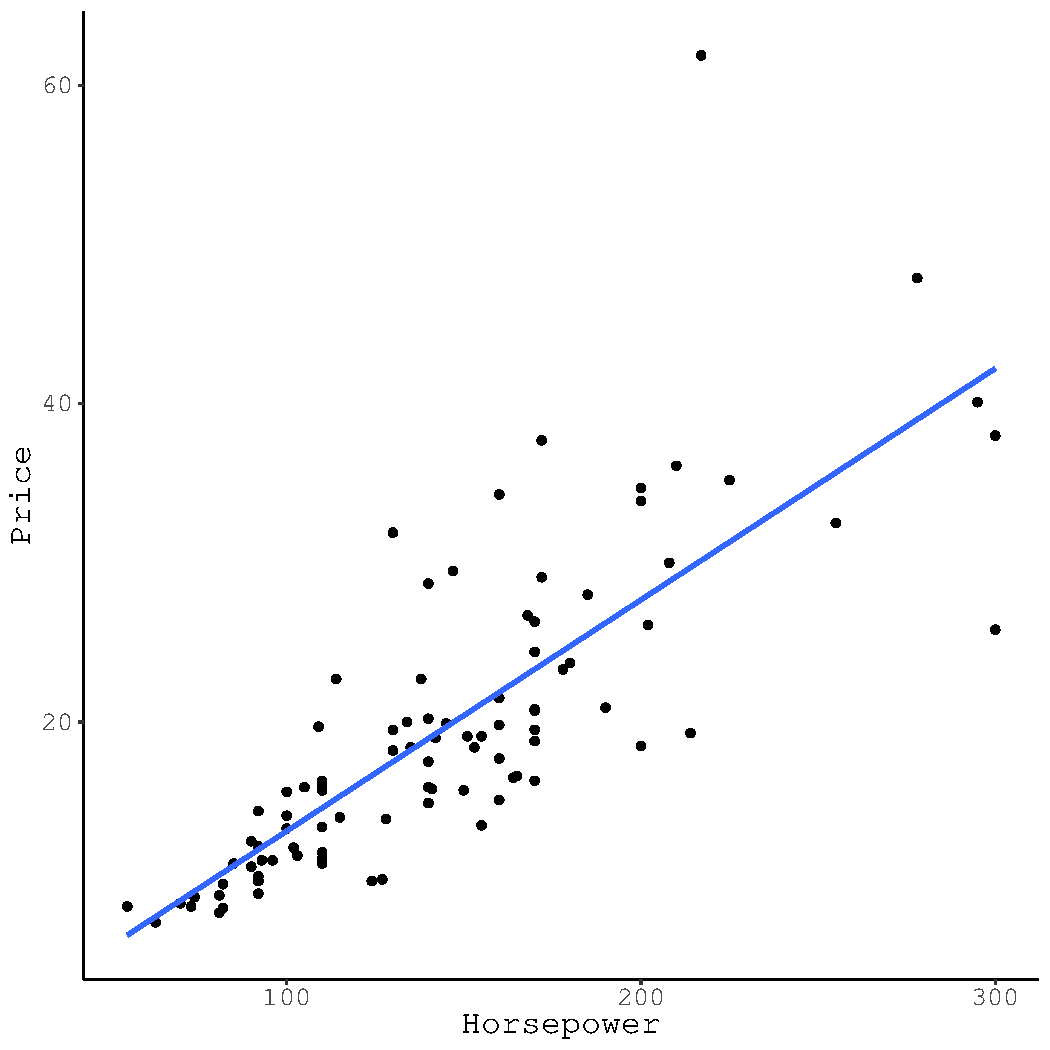
\includegraphics[width=\maxwidth]{figure/assumptions-unnamed-chunk-1-1} 

}


\end{knitrout}
\end{column}
\begin{column}{0.5\textwidth}

\begin{knitrout}\footnotesize
\definecolor{shadecolor}{rgb}{0.878, 0.918, 0.933}\color{fgcolor}

{\centering 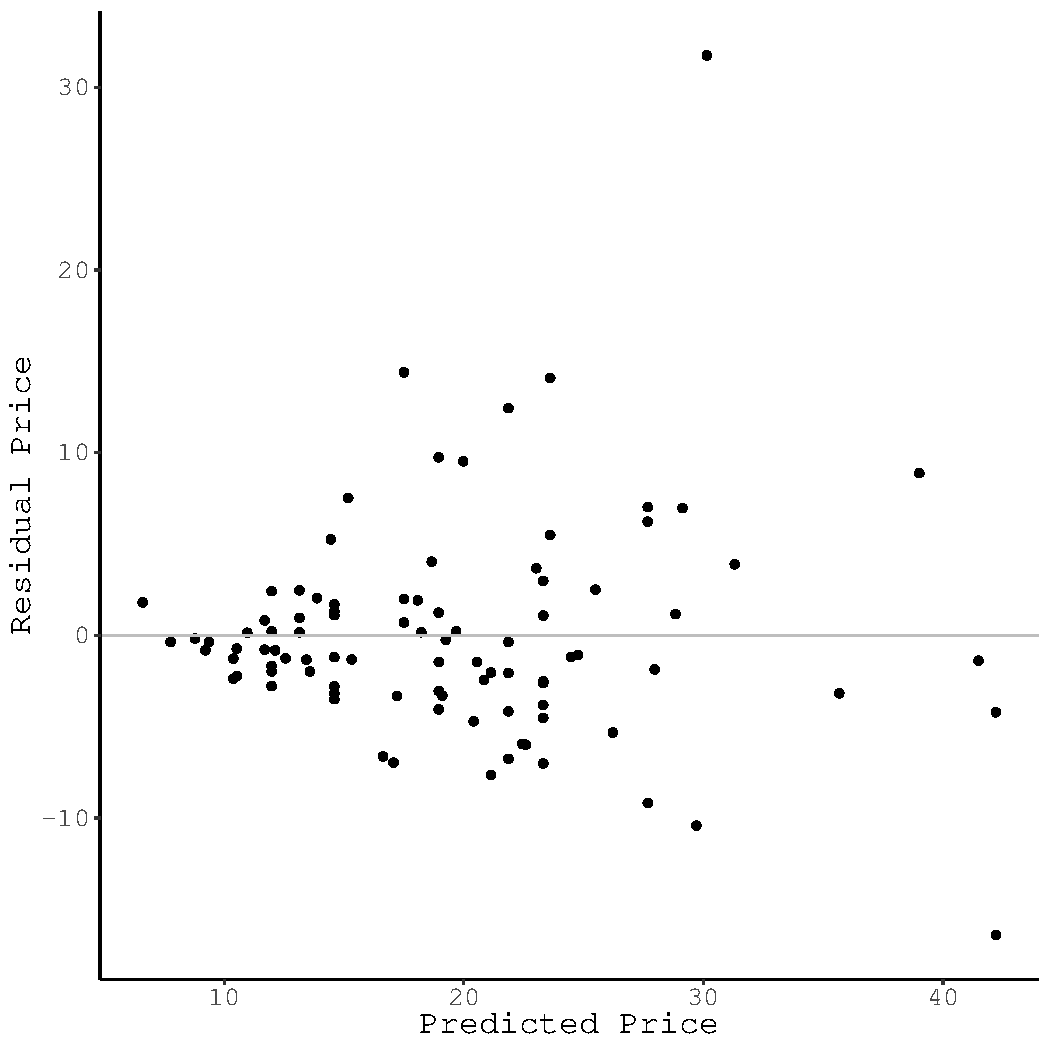
\includegraphics[width=\maxwidth]{figure/assumptions-unnamed-chunk-2-1} 

}


\end{knitrout}
\comment{%%%%%%%%%%%%%%%%%%%%%%%%%%%%%%%%%%%%%%%%%%%%%%%%%%%%%%%%%%%%%%%%%%%%%%%
\begin{knitrout}\footnotesize
\definecolor{shadecolor}{rgb}{0.878, 0.918, 0.933}\color{fgcolor}

{\centering 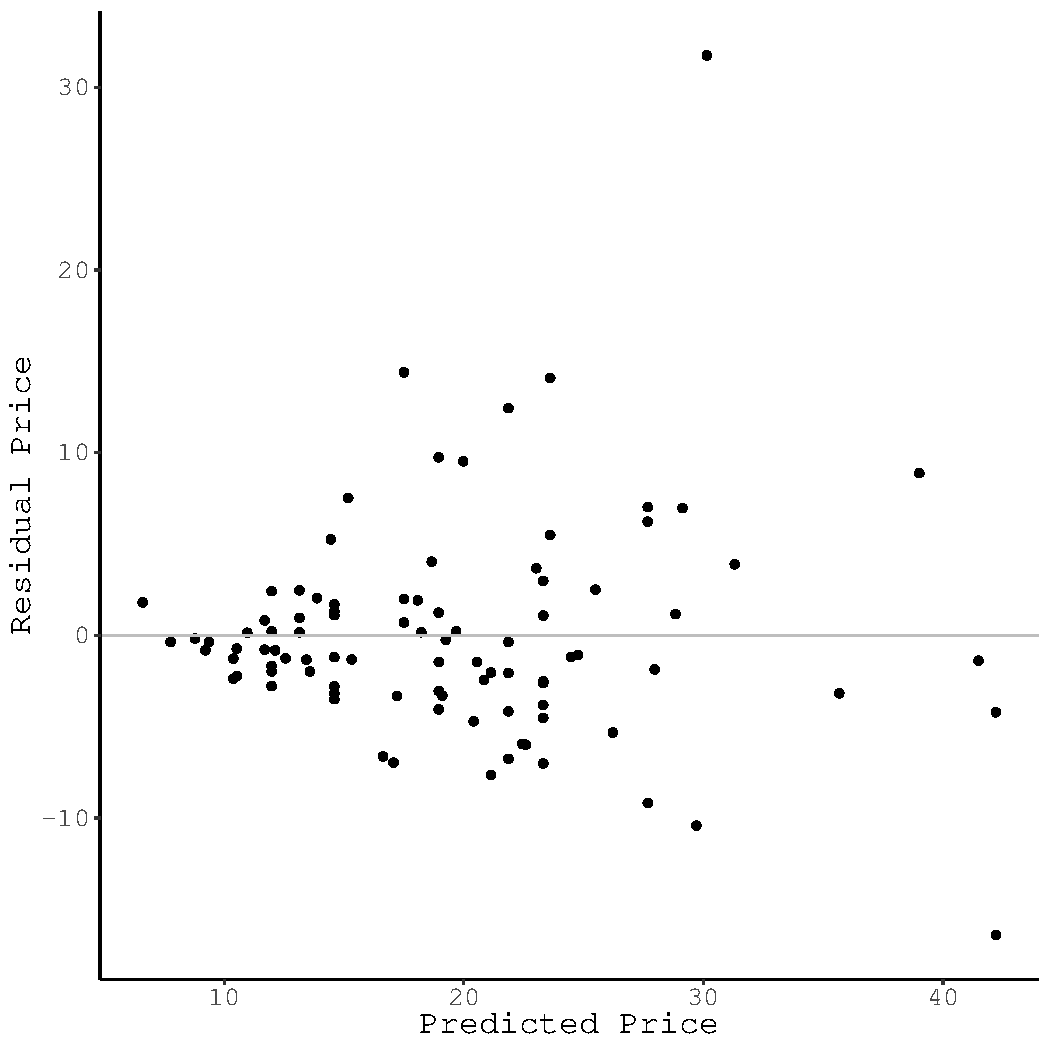
\includegraphics[width=\maxwidth]{figure/assumptions-unnamed-chunk-3-1} 

}


\end{knitrout}
\end{column}

\begin{column}{0.5\textwidth}

\begin{knitrout}\footnotesize
\definecolor{shadecolor}{rgb}{0.878, 0.918, 0.933}\color{fgcolor}

{\centering 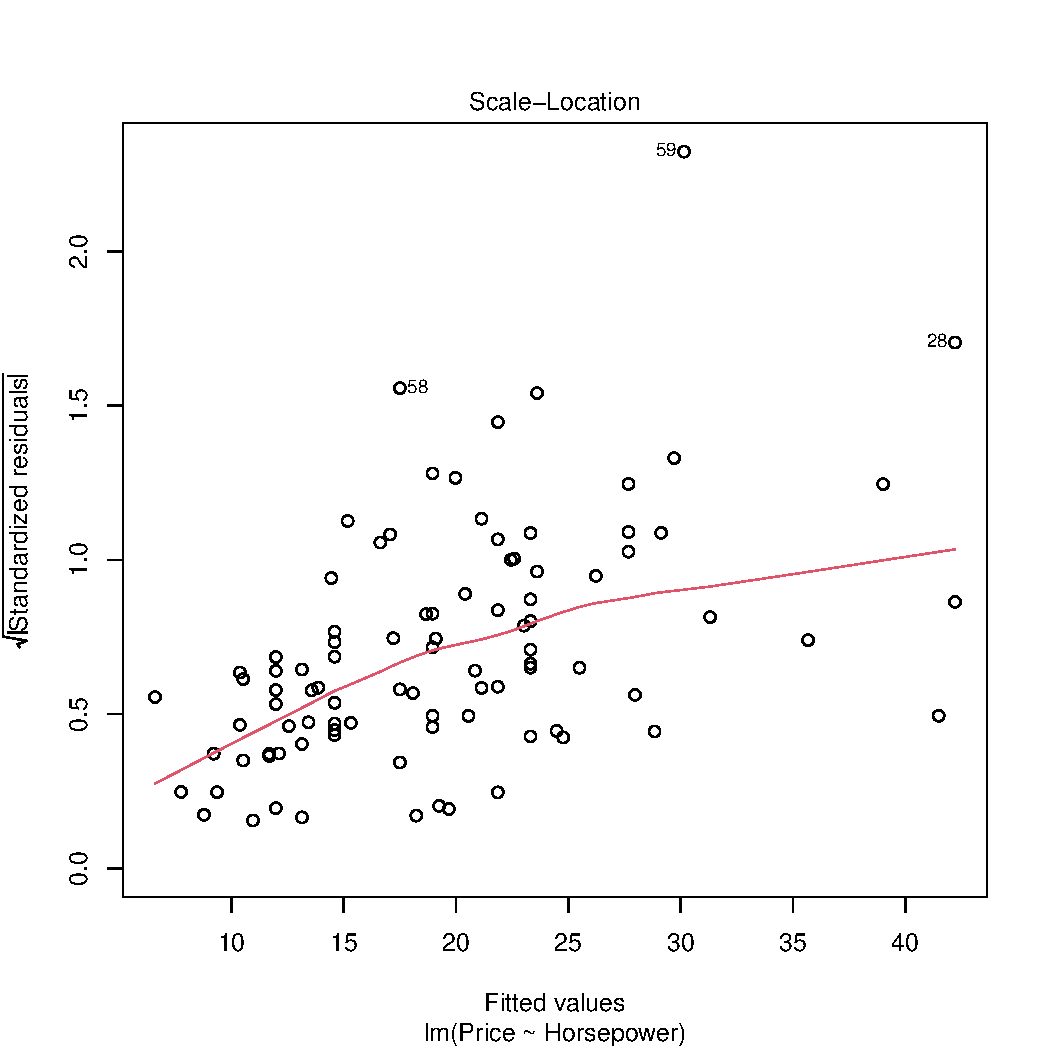
\includegraphics[width=\maxwidth]{figure/assumptions-unnamed-chunk-4-1} 

}


\end{knitrout}
}%%%%%%%%%%%%%%%%%%%%%%%%%%%%%%%%%%%%%%%%%%%%%%%%%%%%%%%%%%%%%%%%%%%%%%%%%%%%%%%
  
\end{column}
\end{columns}

\end{frame}

%------------------------------------------------------------------------------%

\begin{frame}{Partial Regression Plots}
  
\end{frame}

%------------------------------------------------------------------------------%
\comment{%%%%%%%%%%%%%%%%%%%%%%%%%%%%%%%%%%%%%%%%%%%%%%%%%%%%%%%%%%%%%%%%%%%%%%%
\begin{frame}{Heteroscedasticity}

  One commonly encountered problem is non-constant error variance (i.e.,
  \emph{heteroscedasticity}) which violates Assumption \ref{constVar}.

  \vb

  \begin{columns}
    \begin{column}{0.5\textwidth}

\begin{knitrout}\footnotesize
\definecolor{shadecolor}{rgb}{0.878, 0.918, 0.933}\color{fgcolor}

{\centering 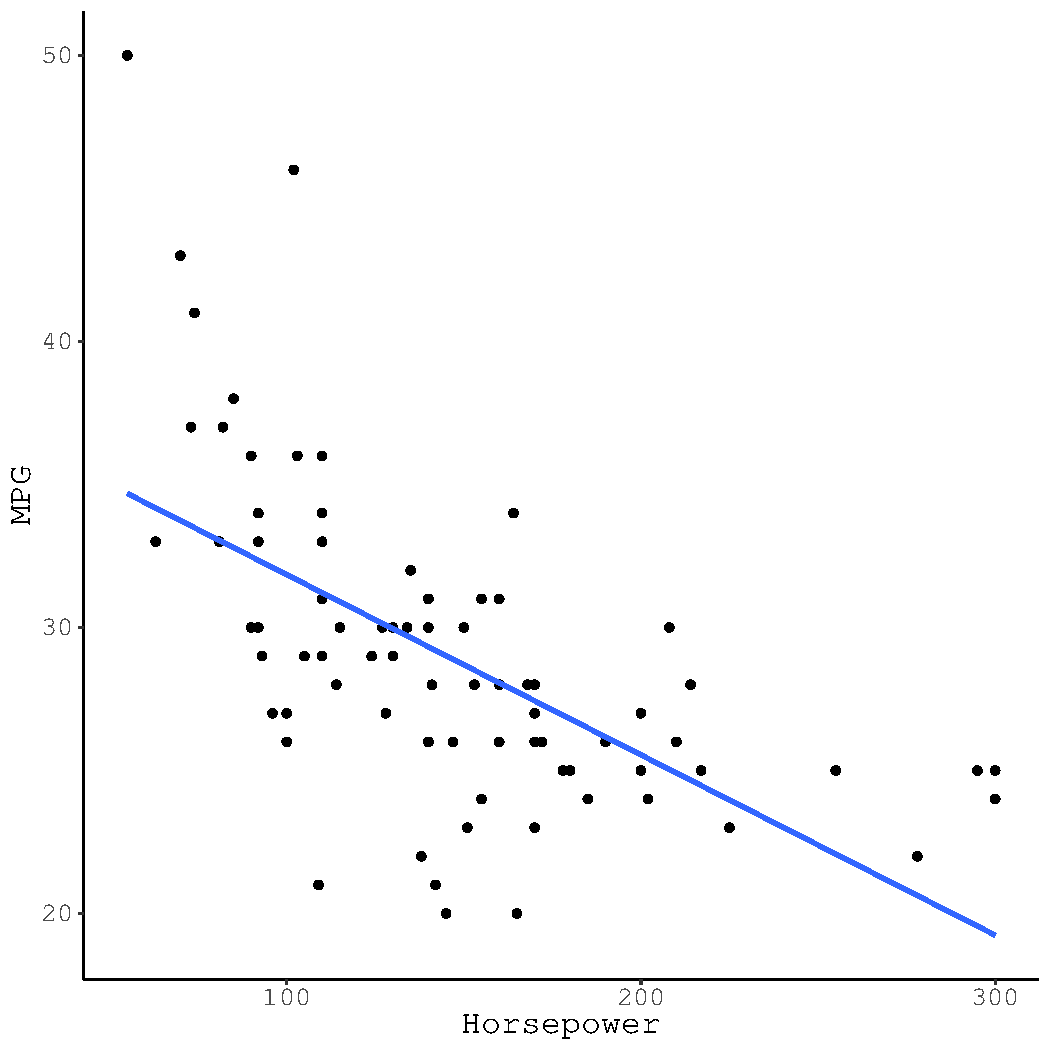
\includegraphics[width=\maxwidth]{figure/assumptions-unnamed-chunk-5-1} 

}


\end{knitrout}
\end{column}
\begin{column}{0.5\textwidth}

\begin{knitrout}\footnotesize
\definecolor{shadecolor}{rgb}{0.878, 0.918, 0.933}\color{fgcolor}

{\centering 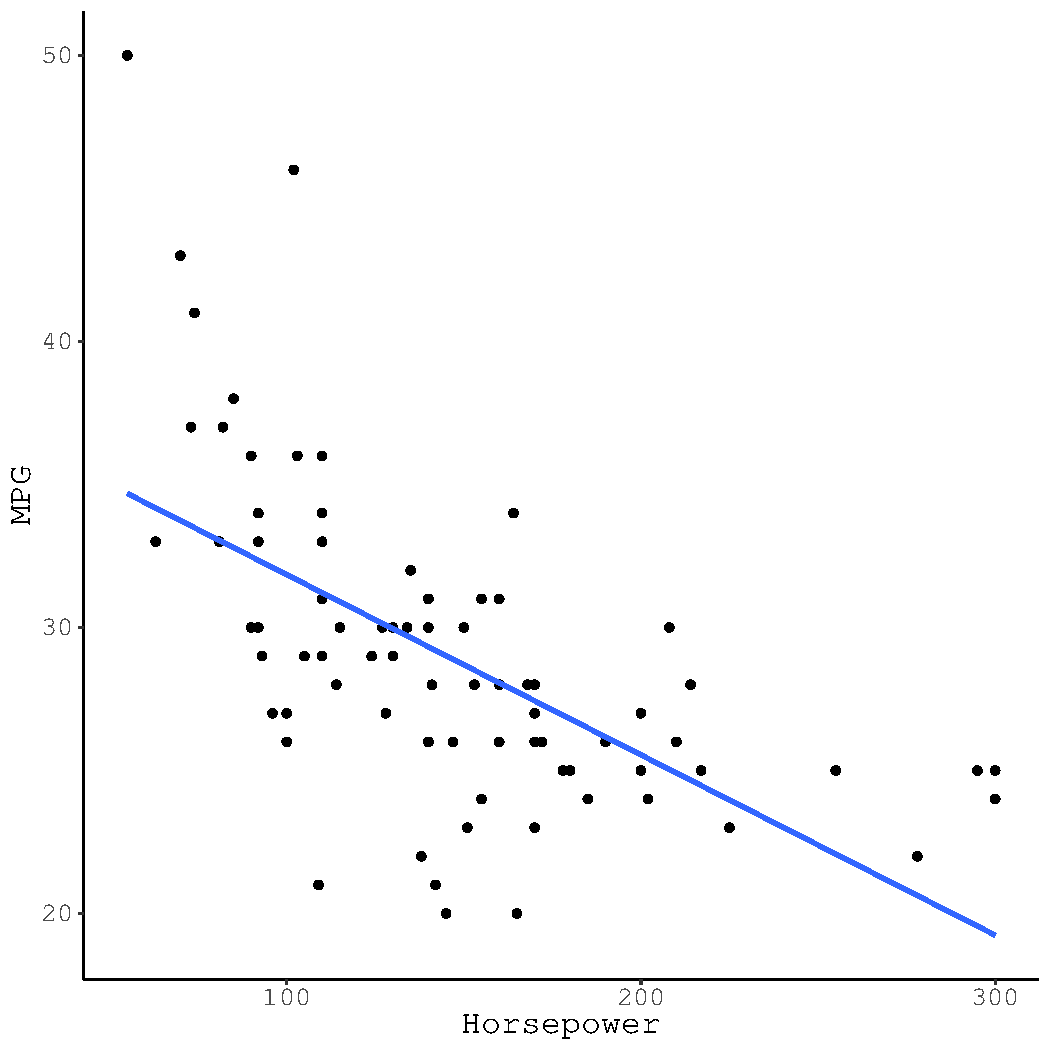
\includegraphics[width=\maxwidth]{figure/assumptions-unnamed-chunk-6-1} 

}


\end{knitrout}

\end{column}
\end{columns}

\end{frame}

%------------------------------------------------------------------------------%

\begin{frame}[fragile]{Heteroscedasticity}

  We can easily generate a simple plot of residuals vs. fitted values by
  plotting the fitted \texttt{lm()} object in R.

  \begin{columns}
    \begin{column}{0.5\textwidth}

\begin{knitrout}\footnotesize
\definecolor{shadecolor}{rgb}{0.878, 0.918, 0.933}\color{fgcolor}\begin{kframe}
\begin{alltt}
\hlstd{out1} \hlkwb{<-} \hlkwd{lm}\hlstd{(Price} \hlopt{~} \hlstd{Horsepower,}
           \hlkwc{data} \hlstd{= Cars93)}

\hlkwd{plot}\hlstd{(out1,} \hlnum{1}\hlstd{)}
\end{alltt}
\end{kframe}
\end{knitrout}

\end{column}
\begin{column}{0.5\textwidth}

\begin{knitrout}\footnotesize
\definecolor{shadecolor}{rgb}{0.878, 0.918, 0.933}\color{fgcolor}

{\centering 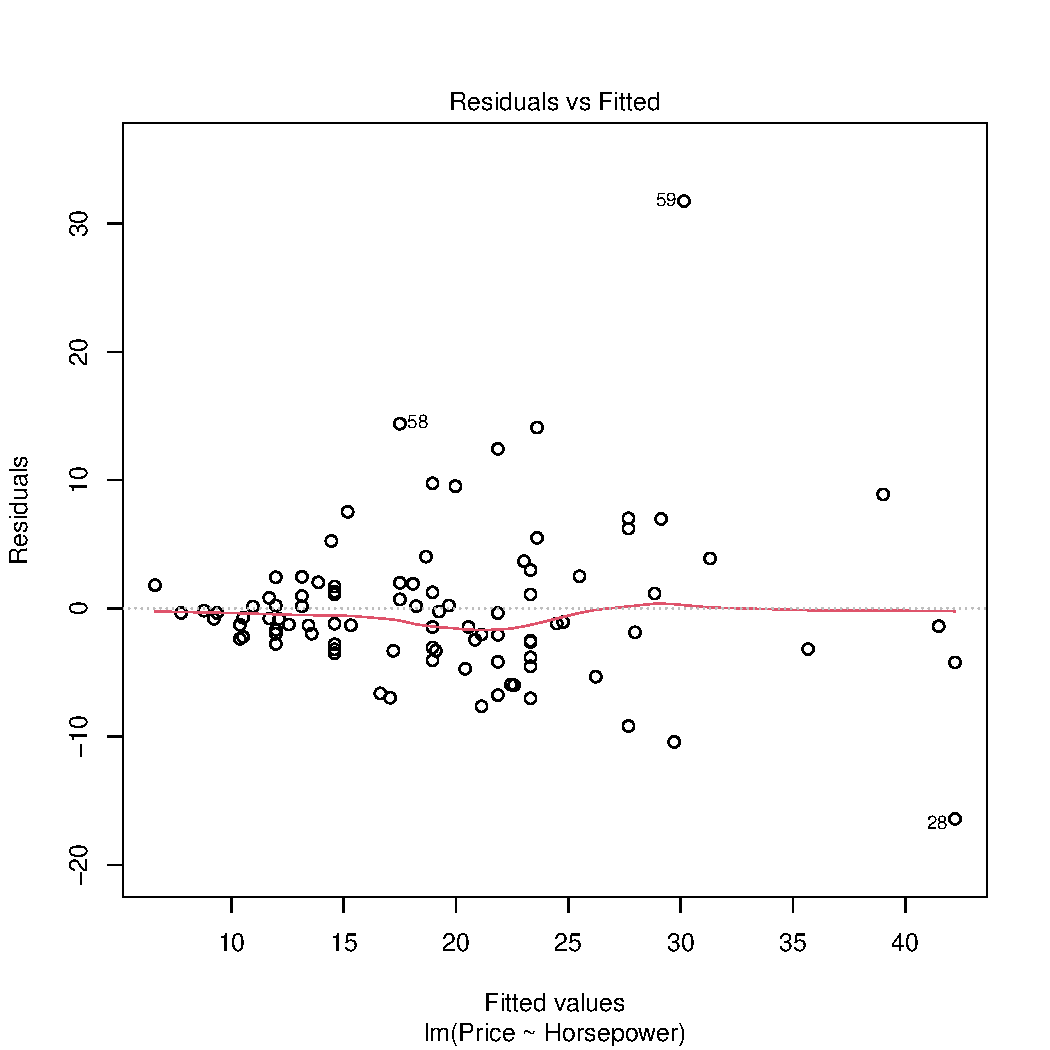
\includegraphics[width=\maxwidth]{figure/assumptions-unnamed-chunk-8-1} 

}


\end{knitrout}

\end{column}
\end{columns}

\end{frame}

\watermarkon %-----------------------------------------------------------------%

\begin{frame}{Consequences of Heteroscedasticity}

  Non-constant error variance will not bias the parameter estimates.
  \begin{itemize}
  \item The best fit line is still correct.
  \item Our measure of uncertainty around that best fit line is wrong.
  \end{itemize}
  \vb
  Heteroscedasticity will bias standard errors (usually downward).
  \begin{itemize}
  \item Test statistics will be too large.
  \item CIs will be too narrow.
  \item We will have inflated Type I error rates.
  \end{itemize}
  \vb
  To get valid inference, we need to address (severe) heteroscedasticity.

\end{frame}

%------------------------------------------------------------------------------%

\begin{frame}{Treating Heteroscedasticity}

  \begin{enumerate}
  \item Transform your outcome using a concave function (e.g., $\ln(Y)$,
    $\sqrt{Y}$).
    \vc
    \begin{itemize}
    \item These transformations will shrink extreme values more than
      small/moderate ones.
    \end{itemize}
    \vb
  \item Refit the model using \emph{weighted least squares}.
    \vc
    \begin{itemize}
    \item Create inverse weights using functions of the residual variances or
      quantities highly correlated therewith.
    \end{itemize}
    \vb
  \item Use a \emph{Heteroscedasticity Consistent} (HC) estimate of the
    asymptotic covariance matrix.
    \vc
    \begin{itemize}
    \item Robust standard errors, Huber-White standard errors, Sandwich
      estimators
    \item HC estimators correct the standard errors for non-constant error
      variance.
    \end{itemize}
  \end{enumerate}

\end{frame}

\watermarkoff %----------------------------------------------------------------%

\begin{frame}[fragile, allowframebreaks]{Example}

\begin{knitrout}\footnotesize
\definecolor{shadecolor}{rgb}{0.878, 0.918, 0.933}\color{fgcolor}\begin{kframe}
\begin{alltt}
\hlcom{## The 'sandwich' package provides several HC estimators:}
\hlkwd{library}\hlstd{(sandwich)}
\end{alltt}


{\ttfamily\noindent\bfseries\color{errorcolor}{Error in library(sandwich): there is no package called 'sandwich'}}\begin{alltt}
\hlcom{## Use sandwich estimator to compute ACOV matrix:}
\hlstd{hcCov} \hlkwb{<-} \hlkwd{vcovHC}\hlstd{(out1)}
\end{alltt}


{\ttfamily\noindent\bfseries\color{errorcolor}{Error in vcovHC(out1): could not find function "{}vcovHC"{}}}\begin{alltt}
\hlcom{## Test coefficients with robust SEs:}
\hlstd{robTest} \hlkwb{<-} \hlkwd{coeftest}\hlstd{(out1,} \hlkwc{vcov} \hlstd{= hcCov)}
\end{alltt}


{\ttfamily\noindent\bfseries\color{errorcolor}{Error in coeftest(out1, vcov = hcCov): could not find function "{}coeftest"{}}}\begin{alltt}
\hlcom{## Test coefficients with default SEs:}
\hlstd{defTest} \hlkwb{<-} \hlkwd{summary}\hlstd{(out1)}\hlopt{$}\hlstd{coefficients}
\end{alltt}
\end{kframe}
\end{knitrout}

\pagebreak

\begin{knitrout}\footnotesize
\definecolor{shadecolor}{rgb}{0.878, 0.918, 0.933}\color{fgcolor}\begin{kframe}
\begin{alltt}
\hlcom{## Compare robust and default approaches:}
\hlstd{robTest}
\end{alltt}


{\ttfamily\noindent\bfseries\color{errorcolor}{Error in eval(expr, envir, enclos): object 'robTest' not found}}\begin{alltt}
\hlstd{defTest}
\end{alltt}
\begin{verbatim}
              Estimate Std. Error    t value     Pr(>|t|)
(Intercept) -1.3987691  1.8200164 -0.7685475 4.441519e-01
Horsepower   0.1453712  0.0118978 12.2183251 6.837464e-21
\end{verbatim}
\end{kframe}
\end{knitrout}

\end{frame}

\watermarkon %-----------------------------------------------------------------%

\begin{frame}{Correlated Errors}

  Errors can become correlated in two basic ways:
  \vb
  \begin{enumerate}
  \item Serial dependence
    \begin{itemize}
    \item When modeling longitudinal data, the errors for a given observational
      unit are correlated over time.
      \vc
    \item We can detect temporal dependence by examining the
      \emph{autocorrelation} of the residuals.
    \end{itemize}
    \vb
  \item Clustering
    \begin{itemize}
    \item Your data have some important, unmodeled, grouping structure.
      \begin{itemize}
      \item Children nested within classrooms
      \item Romantic couples
      \item Departments within a company
      \end{itemize}
      \vc
    \item We can detect problematic levels of clustering with the
      \emph{intraclass correlation coefficient} (ICC).
      \begin{itemize}
      \item We need to know the clustering variable to apply the ICC.
      \end{itemize}
    \end{itemize}
  \end{enumerate}

\end{frame}

%------------------------------------------------------------------------------%

\begin{frame}[allowframebreaks]{Treating Correlated Errors}

  Serially dependent errors in a longitudinal model usually indicate an
  inadequate model.
  \vc
  \begin{itemize}
  \item Your model is ignoring some important aspect of the temporal variation
    that is being absorbed by the error terms.
    \vc
  \item Hopefully, you can add the missing component to your model.
  \end{itemize}

  \pagebreak

  Clustering can be viewed as theoretically meaningful or as a nuisance factor
  that just needs to be controlled.
  \vb
  \begin{itemize}
  \item If the clustering is meaningful, you should model the data using
    \emph{multilevel modeling}.
    \vc
    \begin{itemize}
    \item Hierarchical linear regression
      \vc
    \item Mixed models
      \vc
    \item Random effects models
    \end{itemize}
    \vc
  \item If the clustering is an uninteresting nuisance, you can use specialized
    HC variance estimators that deal with clustering.
  \end{itemize}

\end{frame}

\watermarkoff %----------------------------------------------------------------%

\begin{frame}{Model Specification}

  Our assumptions mostly focus on the errors, so incorrect model specification
  can lead to violations of many assumptions.
  \vb
  \begin{columns}
    \begin{column}{0.5\textwidth}

\begin{knitrout}\footnotesize
\definecolor{shadecolor}{rgb}{0.878, 0.918, 0.933}\color{fgcolor}

{\centering 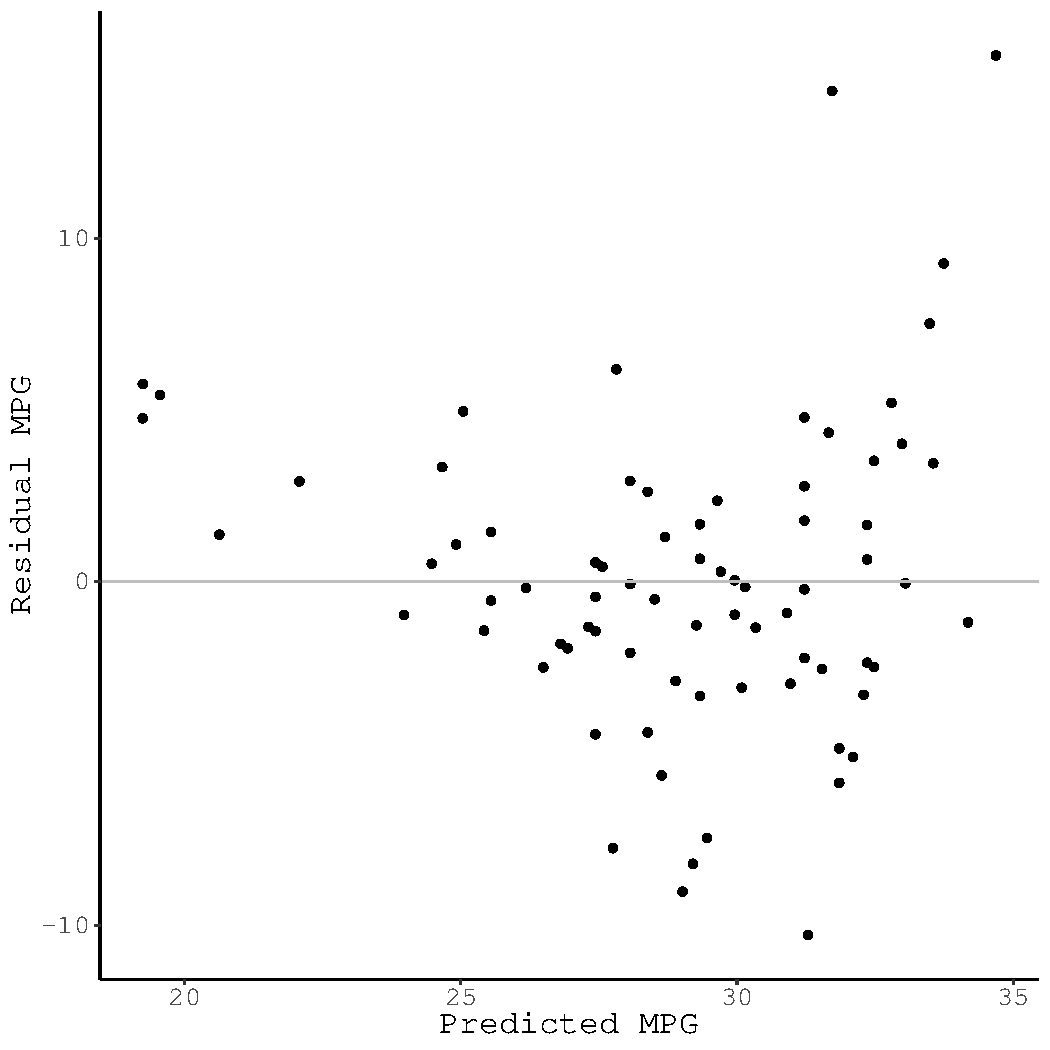
\includegraphics[width=\maxwidth]{figure/assumptions-unnamed-chunk-11-1} 

}


\end{knitrout}

\end{column}

\begin{column}{0.5\textwidth}

\begin{knitrout}\footnotesize
\definecolor{shadecolor}{rgb}{0.878, 0.918, 0.933}\color{fgcolor}

{\centering 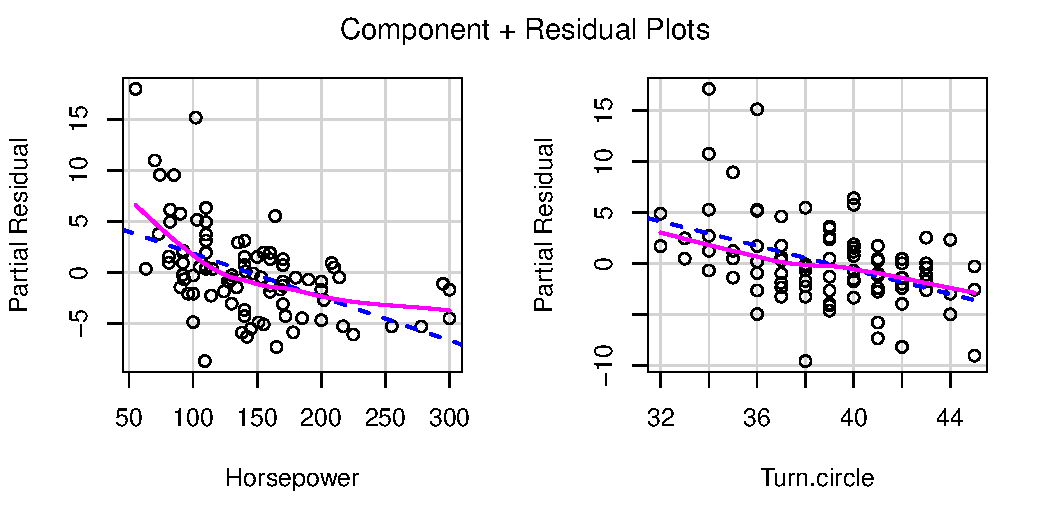
\includegraphics[width=\maxwidth]{figure/assumptions-unnamed-chunk-12-1} 

}


\end{knitrout}

\end{column}
\end{columns}

\end{frame}

%------------------------------------------------------------------------------%

\begin{frame}{Nonlinear Trends in Residual Plots}

  Clearly, the linear trend fits these data poorly.
  \begin{itemize}
    \item We should probably add some polynomial terms
  \end{itemize}
  \vb
  \begin{columns}
    \begin{column}{0.5\textwidth}

\begin{knitrout}\footnotesize
\definecolor{shadecolor}{rgb}{0.878, 0.918, 0.933}\color{fgcolor}

{\centering 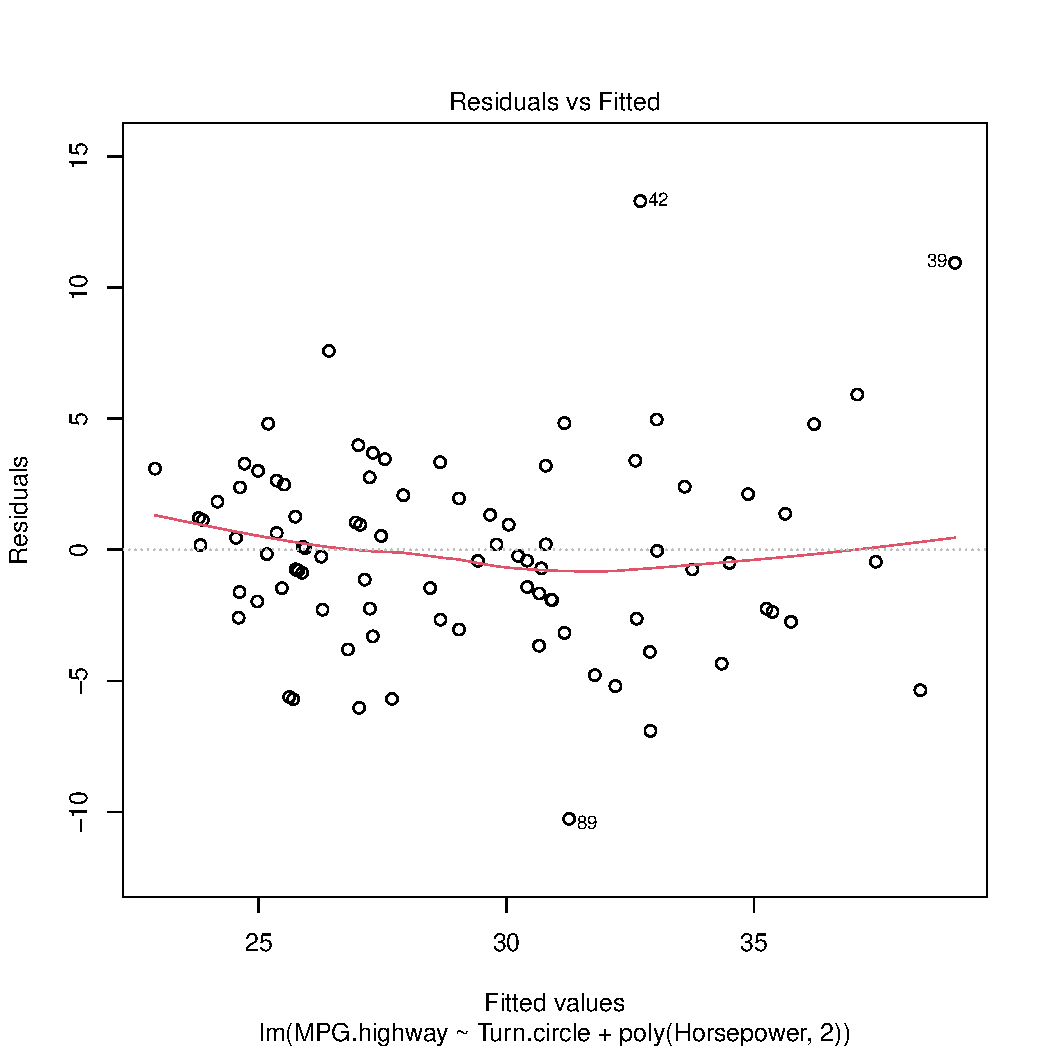
\includegraphics[width=\maxwidth]{figure/assumptions-unnamed-chunk-13-1} 

}


\end{knitrout}

\end{column}

\begin{column}{0.5\textwidth}

\begin{knitrout}\footnotesize
\definecolor{shadecolor}{rgb}{0.878, 0.918, 0.933}\color{fgcolor}

{\centering 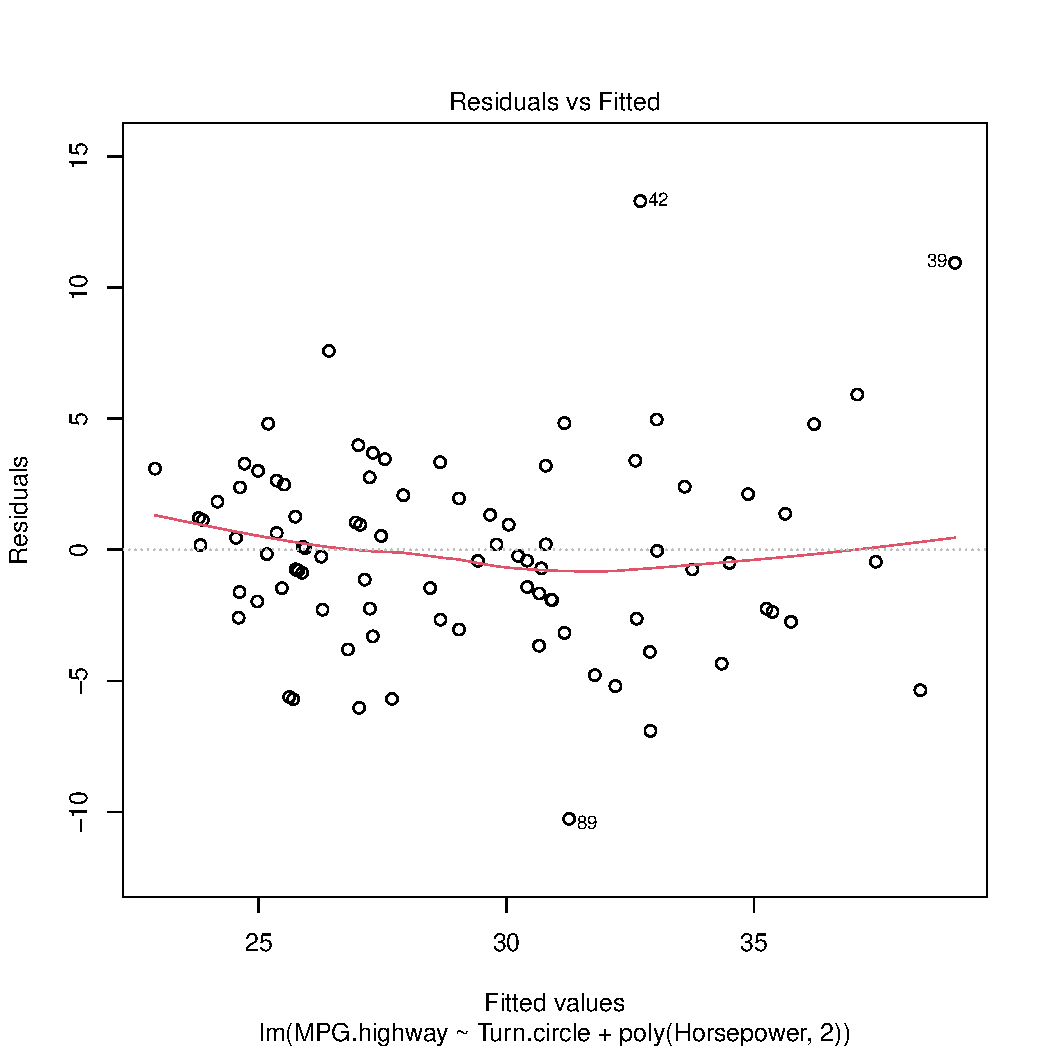
\includegraphics[width=\maxwidth]{figure/assumptions-unnamed-chunk-14-1} 

}


\end{knitrout}

\end{column}
\end{columns}

\end{frame}

\watermarkon %-----------------------------------------------------------------%

\begin{frame}{Treating Residual Nonlinearity}

  Nonlinearity in the residual plots is usually a sign of either:
  \begin{enumerate}
  \item Model misspecification
  \item Influential observations
  \end{enumerate}
  \vb
  This type of model misspecification usually implies omitted functions of
  modeled variables.
  \begin{itemize}
  \item Polynomial terms
  \item Interactions
  \end{itemize}
  \vb
  The solution is to include the omitted term into the model and refit.
  \begin{itemize}
  \item This is very much easier said than done.
  \end{itemize}

\end{frame}

\watermarkoff %----------------------------------------------------------------%

\begin{frame}{Residual Plots}

  Certainly looks better, but not ideal.
  \vb
  \begin{columns}
    \begin{column}{0.5\textwidth}

\begin{knitrout}\footnotesize
\definecolor{shadecolor}{rgb}{0.878, 0.918, 0.933}\color{fgcolor}

{\centering 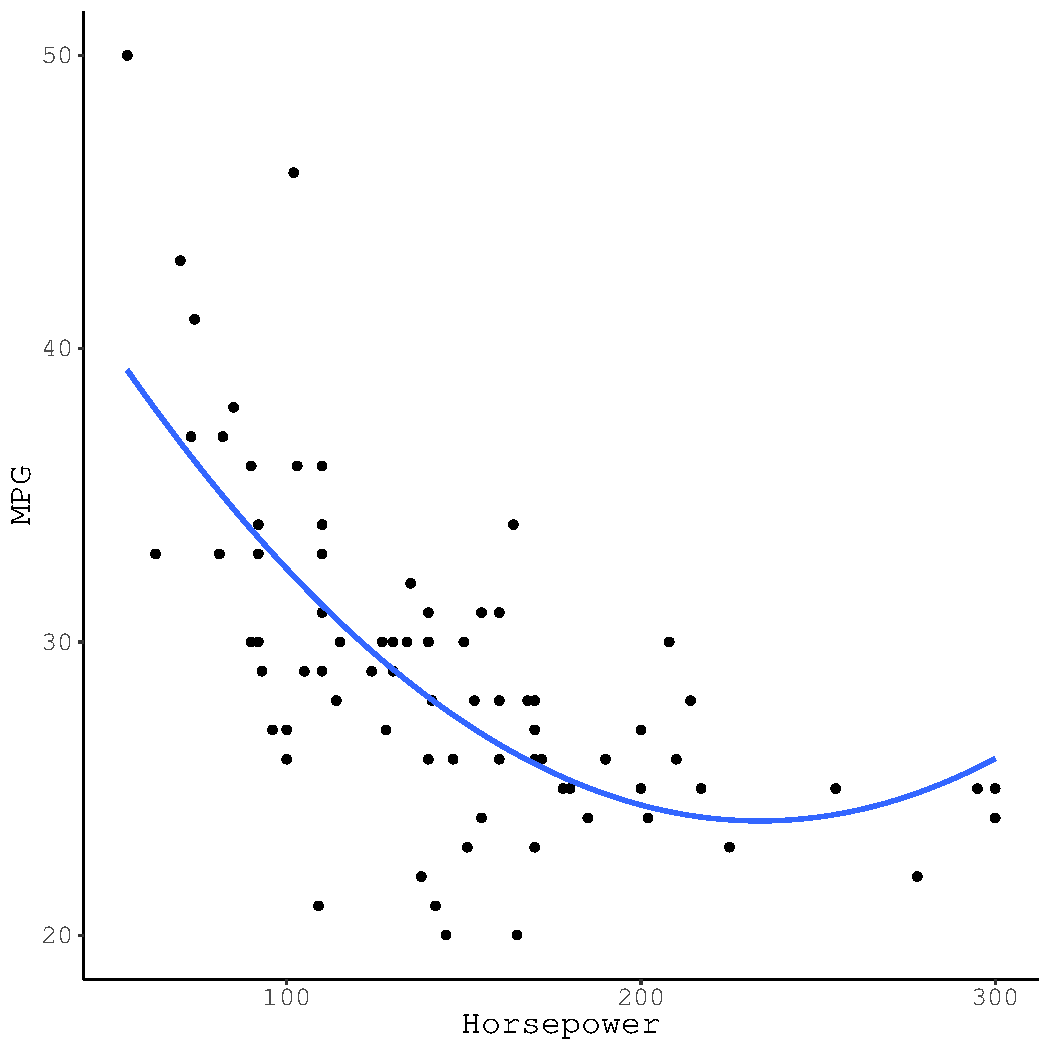
\includegraphics[width=\maxwidth]{figure/assumptions-unnamed-chunk-15-1} 

}


\end{knitrout}

\end{column}

\begin{column}{0.5\textwidth}

\begin{knitrout}\footnotesize
\definecolor{shadecolor}{rgb}{0.878, 0.918, 0.933}\color{fgcolor}

{\centering 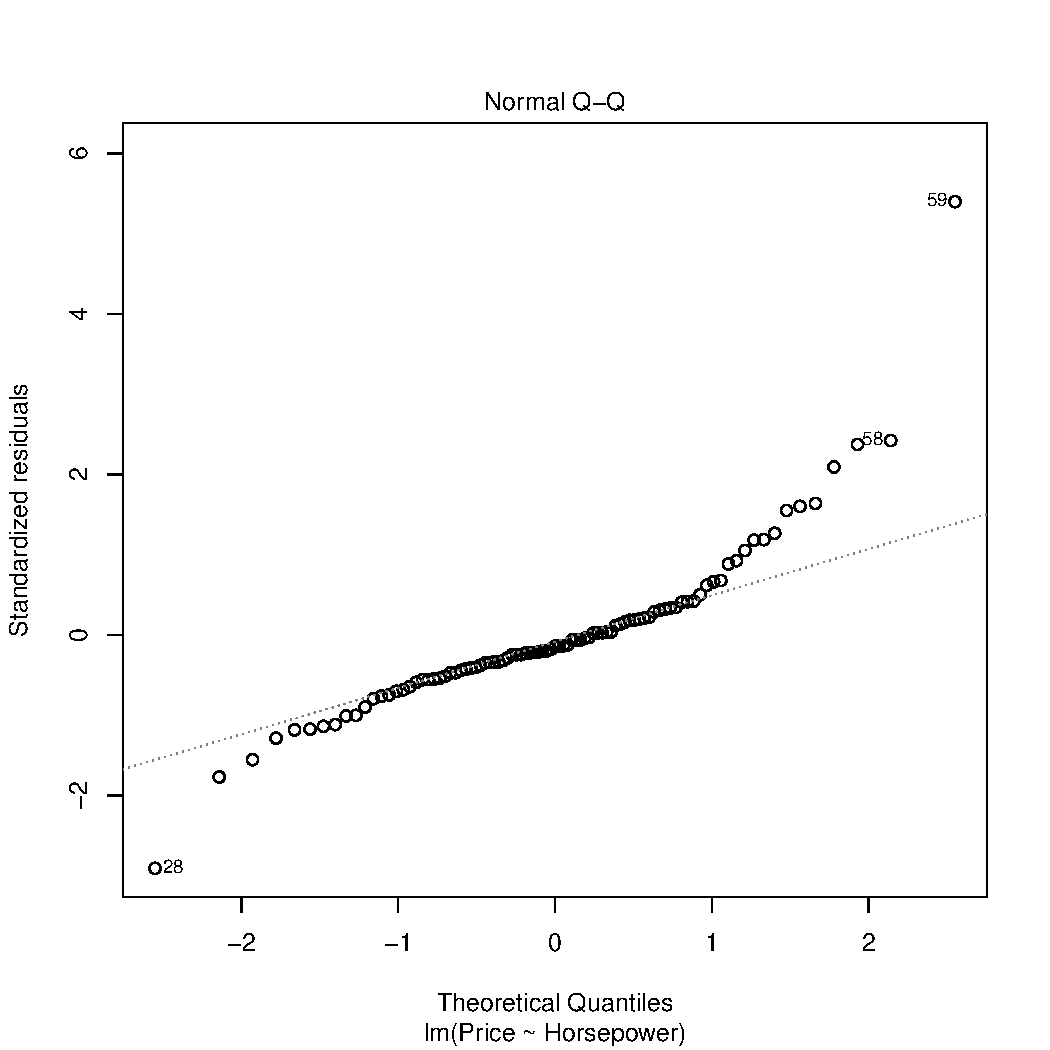
\includegraphics[width=\maxwidth]{figure/assumptions-unnamed-chunk-16-1} 

}


\end{knitrout}

\end{column}
\end{columns}

\end{frame}

%------------------------------------------------------------------------------%

\begin{frame}{Residual Plots}

  Further improvement (perhaps).
  \vb
  \begin{columns}
    \begin{column}{0.5\textwidth}

\begin{knitrout}\footnotesize
\definecolor{shadecolor}{rgb}{0.878, 0.918, 0.933}\color{fgcolor}

{\centering 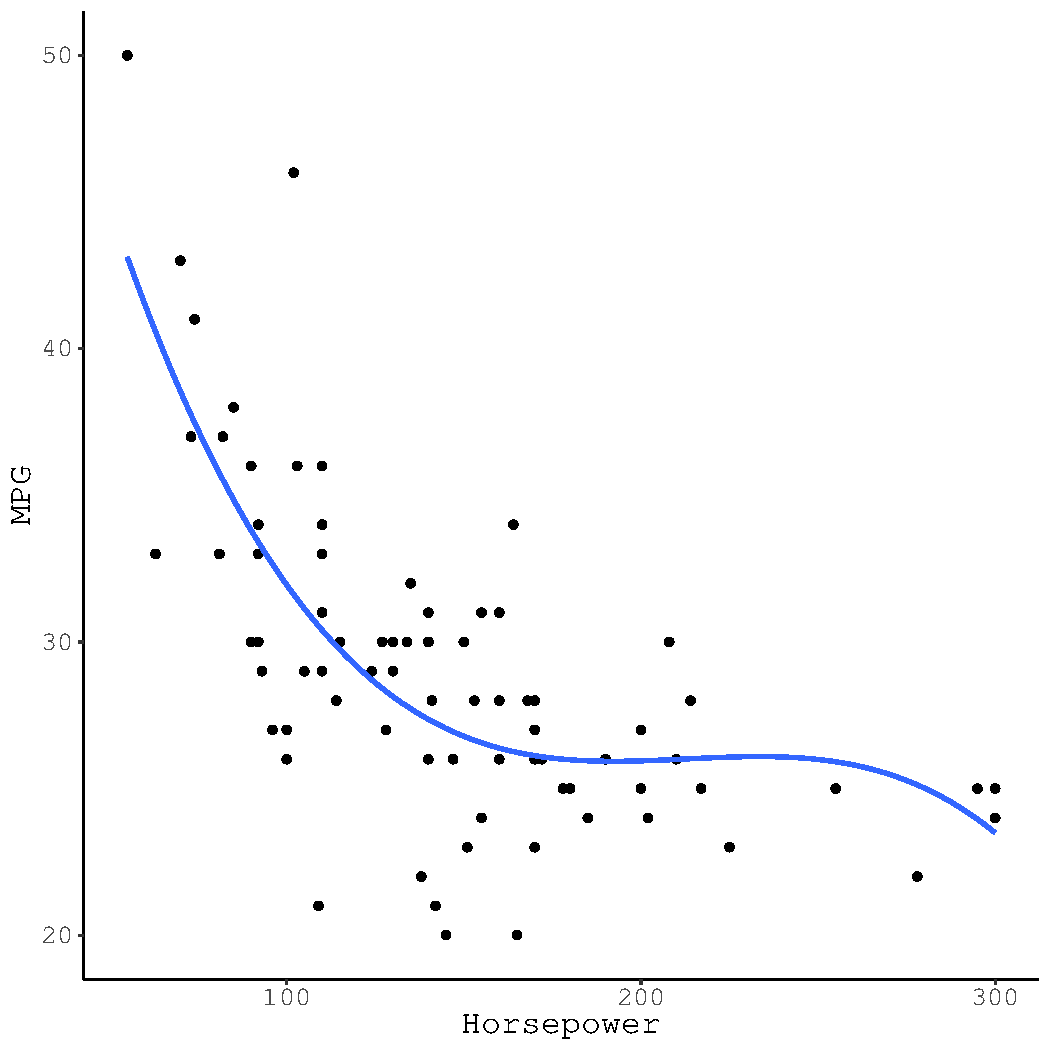
\includegraphics[width=\maxwidth]{figure/assumptions-unnamed-chunk-17-1} 

}


\end{knitrout}

\end{column}

\begin{column}{0.5\textwidth}

\begin{knitrout}\footnotesize
\definecolor{shadecolor}{rgb}{0.878, 0.918, 0.933}\color{fgcolor}

{\centering 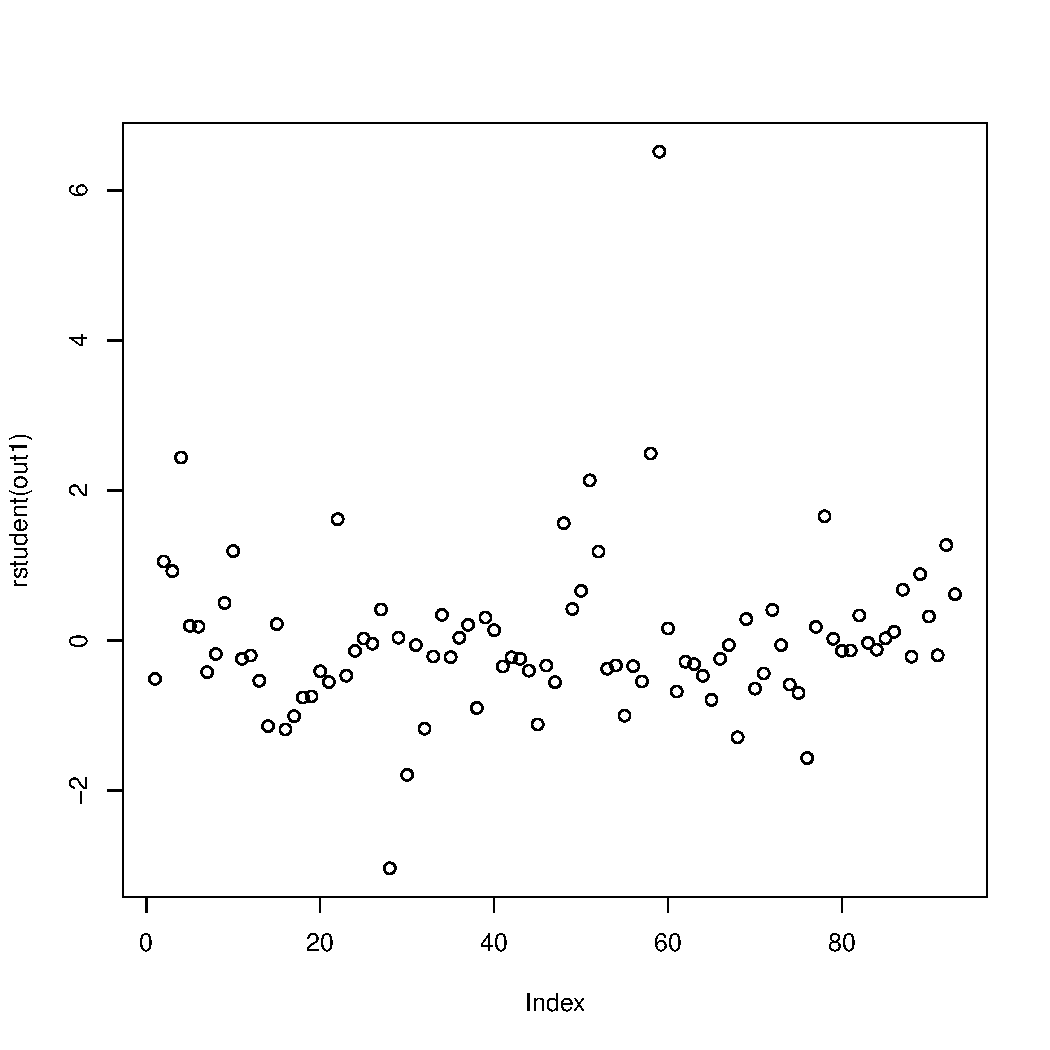
\includegraphics[width=\maxwidth]{figure/assumptions-unnamed-chunk-18-1} 

}


\end{knitrout}

\end{column}
\end{columns}

\end{frame}

\watermarkon %-----------------------------------------------------------------%

\begin{frame}[allowframebreaks]{Omitted Variables}

  The most common cause of endogeneity (i.e., violating Assumption \ref{exo}) is
  \emph{omitted variable bias}.
  \vb
  \begin{itemize}
  \item If we leave an important predictor variable out of our equation, some
    modeled predictors will become endogenous and their estimated regression
    slopes will be biased.
    \vb
  \item The omitted variable must be correlated with $Y$ and at least one of the
    modeled $X_p$, to be a problem.
  \end{itemize}

  \pagebreak

  Assume the following is the true regression model.
  \begin{align*}
    Y = \beta_0 + \beta_1X + \beta_2Z + \varepsilon
  \end{align*}
  Now, suppose we omit $Z$ from the model:
  \begin{align*}
    Y &= \beta_0 + \beta_1X + \omega\\
    \omega &= \varepsilon + \beta_2Z
  \end{align*}
  Our new error, $\omega$, is a combination of the true error, $\varepsilon$,
  and the omitted term, $\beta_2Z$.
  \begin{itemize}
  \item Consequently, if $X$ and $Z$ are correlated, omitting $Z$ induces a
    correlation between $X$ and $\omega$ (i.e., endogeneity).
  \end{itemize}

\end{frame}

%------------------------------------------------------------------------------%

\begin{frame}{Treating Omitted Variable Bias}

  Omitted variable bias can have severe consequences, but you can't really test
  for it.
  \vb
  \begin{itemize}
  \item The \emph{errors} are correlated with the predictors, but our model is
    estimated under the assumption of exogeneity, so the \emph{residuals} from
    our model will generally be uncorrelated with the predictors.
    \vb
  \item We mostly have to pro-actively work to include all relevant variables in
    our model.
  \end{itemize}

\end{frame}

\watermarkoff %----------------------------------------------------------------%
}%%%%%%%%%%%%%%%%%%%%%%%%%%%%%%%%%%%%%%%%%%%%%%%%%%%%%%%%%%%%%%%%%%%%%%%%%%%%%%%

\begin{frame}{QQ-Plot}
  
  \begin{columns}
    \begin{column}{0.5\textwidth}

      One of the best ways to evaluate the normality of the error distribution
      with a Q-Q Plot.
      \vc
      \begin{itemize}
      \item Plot the quantiles of the residual distribution against the
        theoretically ideal quantiles.
        \vc
      \item We can actually use a Q-Q Plot to compare any two distributions.
      \end{itemize}

    \end{column}

    \begin{column}{0.5\textwidth}

\begin{knitrout}\footnotesize
\definecolor{shadecolor}{rgb}{0.878, 0.918, 0.933}\color{fgcolor}\begin{kframe}
\begin{alltt}
\hlkwd{plot}\hlstd{(out1,} \hlnum{2}\hlstd{)}
\end{alltt}
\end{kframe}

{\centering 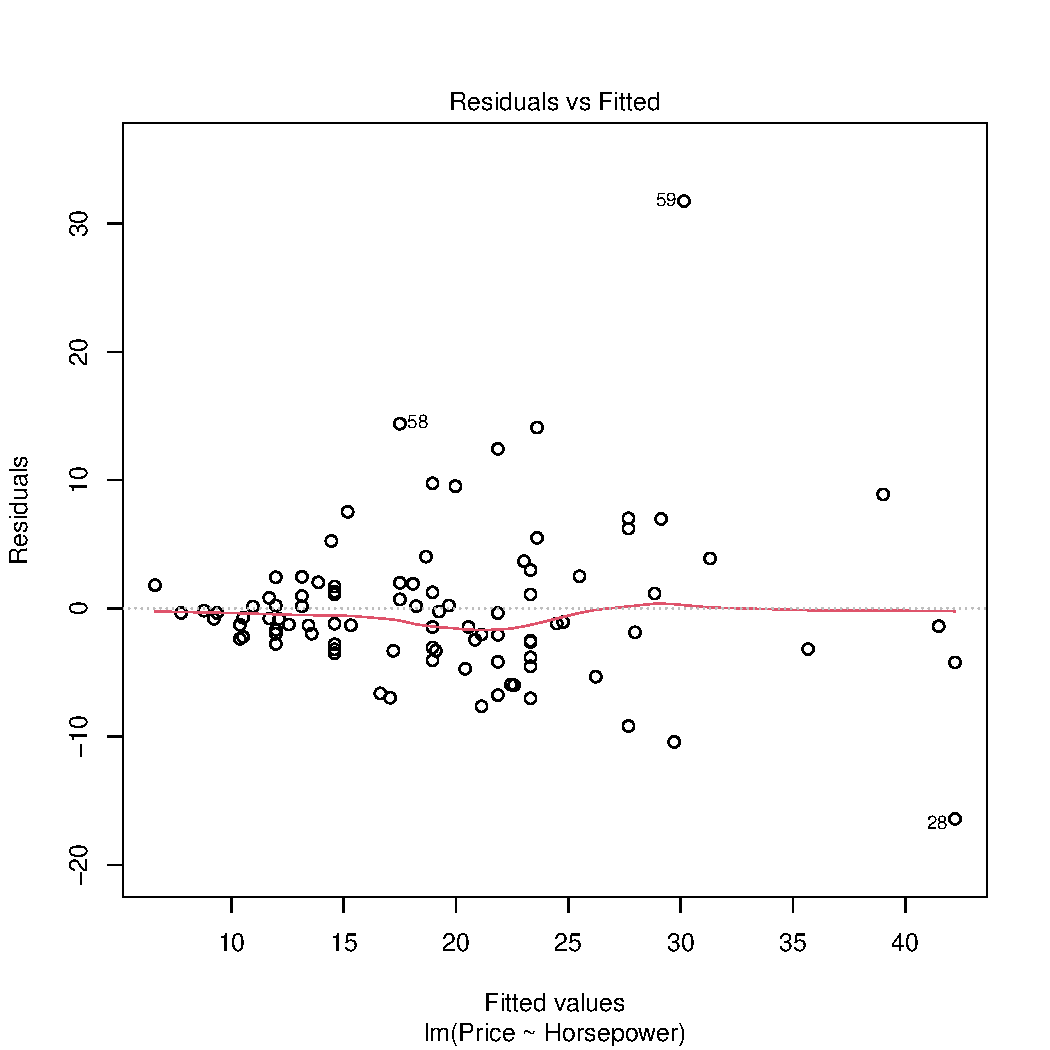
\includegraphics[width=\maxwidth]{figure/assumptions-unnamed-chunk-19-1} 

}


\end{knitrout}



    \end{column}
  \end{columns}

\end{frame}

\watermarkon %-----------------------------------------------------------------%
\comment{%%%%%%%%%%%%%%%%%%%%%%%%%%%%%%%%%%%%%%%%%%%%%%%%%%%%%%%%%%%%%%%%%%%%%%%
\begin{frame}{Consequences of Violating Normality}

  In small samples, with \emph{\underline{fixed}} predictors, normally
  distributed errors imply normal sampling distributions for the regression
  coefficients.
  \vc
  \begin{itemize}
  \item In large samples, the central limit theorem implies normal sampling
    distributions for the coefficients, regardless of the error distribution.
  \end{itemize}
  \va
  \pause
  Prediction intervals require normally distributed errors.
  \vc
  \begin{itemize}
  \item Confidence intervals for predictions share the same normality
    requirements as the coefficients' sampling distributions.
  \end{itemize}

\end{frame}

%------------------------------------------------------------------------------%

\begin{frame}{Treating Violations of Normality}

  We usually don't need to do anything about non-normal errors.
  \begin{itemize}
  \item The CLT will protect our inferences.
  \end{itemize}
  \vb
  \pause
  We can use \emph{bootstrapping} to get around the need for normality.
  \begin{enumerate}
  \item Treat your sample as a synthetic population from which you draw many new
    samples (with replacement).
  \item Estimate your model in each new sample.
  \item The replicates of your estimated parameters generate an empirical
    sampling distribution that you can use for inference.
  \end{enumerate}
  \vb
  \pause
  Bootstrapping can be used for inference on pretty much any estimable
  parameter, but it won't work with small samples.
  \begin{itemize}
  \item Need to assume that your sample is representative of the population
  \end{itemize}

\end{frame}
}%%%%%%%%%%%%%%%%%%%%%%%%%%%%%%%%%%%%%%%%%%%%%%%%%%%%%%%%%%%%%%%%%%%%%%%%%%%%%%%
%------------------------------------------------------------------------------%

\sectionslide{Influential Observations}

%------------------------------------------------------------------------------%

\begin{frame}{Influential Observations}

  Influential observations contaminate analyses in two ways:
  \vc
  \begin{enumerate}
  \item Exert too much influence on the fitted regression model
    \vc
  \item Invalidate estimates/inferences by violating assumptions
  \end{enumerate}
  \vb
  There are two distinct types of influential observations:
  \vc
  \begin{enumerate}
  \item Outliers
    \vc
    \begin{itemize}
    \item Observations with extreme outcome values, relative to the other data.
      \vc
    \item Observations with outcome values that fit the model very badly.
    \end{itemize}
    \vb
  \item High-leverage observations
    \vc
    \begin{itemize}
    \item Observation with extreme predictor values, relative to other data.
    \end{itemize}
  \end{enumerate}

\end{frame}

%------------------------------------------------------------------------------%

\begin{frame}{Outliers}

  Outliers can be identified by scrutinizing the residuals.
  \vc
  \begin{itemize}
  \item Observations with residuals of large magnitude may be outliers.
    \vc
  \item The difficulty arises in quantifying what constitutes a ``large''
    residual.
  \end{itemize}
  \vb
  If the residuals do not have constant variance, then we cannot directly
  compare them.
  \vc
  \begin{itemize}
  \item We need to standardize the residuals in some way.
  \end{itemize}

\end{frame}

%------------------------------------------------------------------------------%

\begin{frame}{Detecting Outliers}

  We are specifically interested in \emph{externally studentized residuals}.
  \vb
  \begin{itemize}
  \item We can't simply standardize the ordinary residuals.
    \begin{itemize}
    \item \emph{Internally studentized residuals}
      \vc
    \item Outliers can pull the regression line towards themselves.
      \vc
    \item The internally studentized residuals for outliers will be too small.
    \end{itemize}
  \end{itemize}
  \vb
  Begin by defining the concept of a \emph{deleted residual}:
  \begin{align*}
    \hat{\varepsilon}_{(n)} = Y_n - \hat{Y}_{(n)}
  \end{align*}
  \vx{-18}
  \begin{itemize}
    \item $\hat{\varepsilon}_{(n)}$ quantifies the distance of $Y_n$ from the
      regression line estimated after excluding the $n$th observation.
  \end{itemize}

\end{frame}

%------------------------------------------------------------------------------%

\begin{frame}{Studentized Residuals}

  If we standardize the deleted residual, $\hat{\varepsilon}_{(n)}$, we get the
  externally studentized residual:
  \begin{align*}
    t_{(n)} = \frac{\hat{\varepsilon}_{(n)}}{SE_{\hat{\varepsilon}_{(n)}}}
  \end{align*}
  The externally studentized residuals have two very useful properties:
  \vb
  \begin{enumerate}
  \item Each $t_{(n)}$ is scaled equivalently.
    \vc
    \begin{itemize}
    \item We can directly compare different $t_{(n)}$.
    \end{itemize}
    \vb
  \item The $t_{(n)}$ are \emph{Student's t} distributed.
    \vc
    \begin{itemize}
    \item We can quantify outliers in terms of quantiles of the $t$
      distribution.
      \vc
    \item $|t_{(n)}| > 3.0$ is a common rule of thumb for flagging outliers.
    \end{itemize}
  \end{enumerate}

\end{frame}

\watermarkoff %----------------------------------------------------------------%

\begin{frame}{Studentized Residual Plots}

  \begin{columns}
    \begin{column}{0.5\textwidth}

      Index plots of the externally studentized residuals can help spotlight
      potential outliers.
      \vb
      \begin{itemize}
      \item Look for observations that clearly ``stand out from the crowd.''
      \end{itemize}

    \end{column}

    \begin{column}{0.5\textwidth}

\begin{knitrout}\footnotesize
\definecolor{shadecolor}{rgb}{0.878, 0.918, 0.933}\color{fgcolor}\begin{kframe}
\begin{alltt}
\hlkwd{plot}\hlstd{(}\hlkwd{rstudent}\hlstd{(out1))}
\end{alltt}
\end{kframe}

{\centering 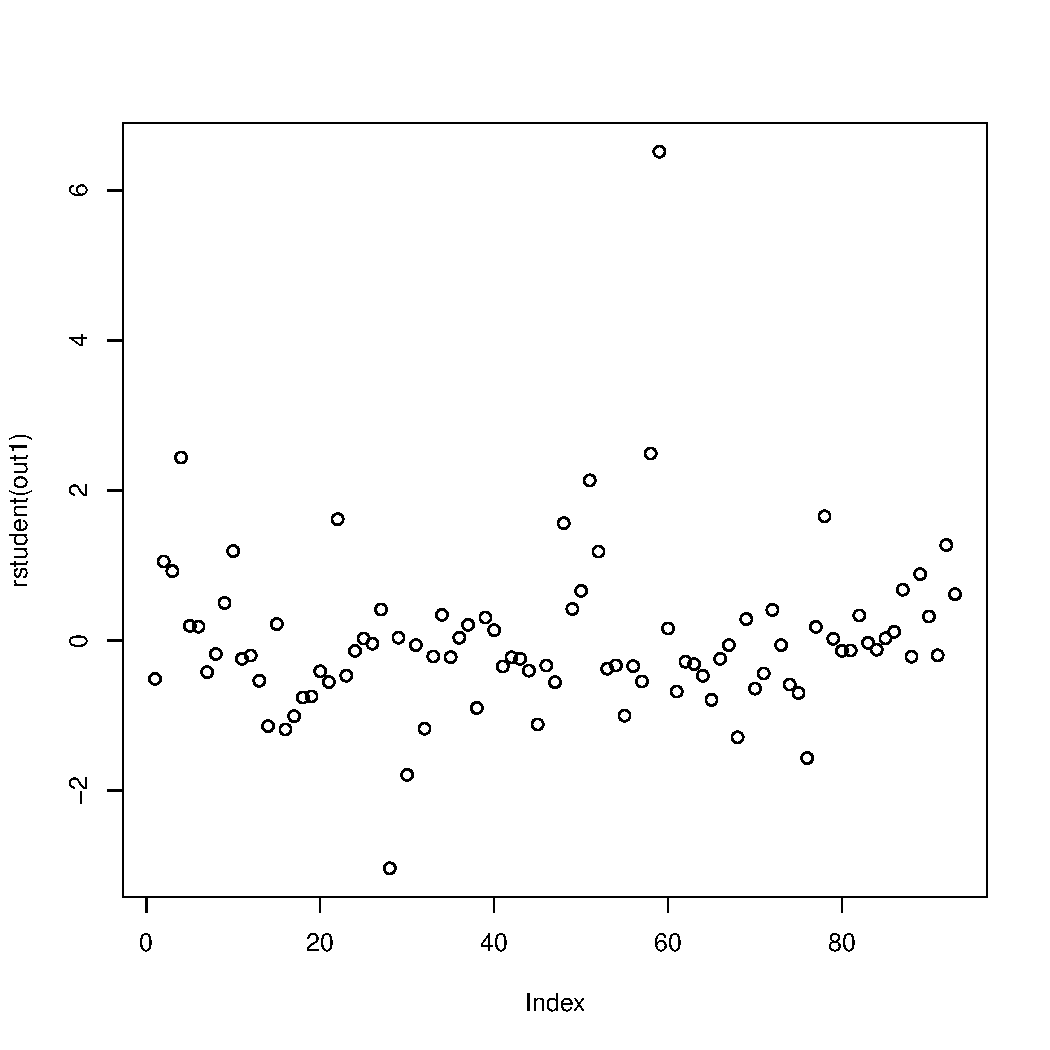
\includegraphics[width=\maxwidth]{figure/assumptions-unnamed-chunk-21-1} 

}


\end{knitrout}



\end{column}
\end{columns}

\end{frame}

\watermarkon %-----------------------------------------------------------------%

\begin{frame}{High-Leverage Points}

  We identify high-leverage observations through their \emph{leverage} values.
  \vb
  \begin{itemize}
  \item An observation's leverage, $h_n$, quantifies the extent to which its
    predictors affect the fitted regression model.
    \vb
  \item Observations with $X$ values very far from the mean, $\bar{X}$, affect
    the fitted model disproportionately.
  \end{itemize}
  \vb
  \pause
  In simple linear regression, the $n$th leverage is given by:
  \begin{align*}
    h_n = \frac{1}{N} + \frac{\left(X_n - \bar{X}\right)^2}
    {\sum_{m = 1}^N \left(X_{m} - \bar{X}\right)^2}
  \end{align*}

\end{frame}

\watermarkoff %----------------------------------------------------------------%

\begin{frame}{Leverage Plots}

  \begin{columns}
    \begin{column}{0.5\textwidth}

      Index plots of the leverage values can help spotlight high-leverage points.
      \vb
      \begin{itemize}
      \item Again, look for observations that clearly ``stand out from the
        crowd.''
      \end{itemize}

    \end{column}

    \begin{column}{0.5\textwidth}

\begin{knitrout}\footnotesize
\definecolor{shadecolor}{rgb}{0.878, 0.918, 0.933}\color{fgcolor}\begin{kframe}
\begin{alltt}
\hlkwd{plot}\hlstd{(}\hlkwd{hatvalues}\hlstd{(out1))}
\end{alltt}
\end{kframe}

{\centering 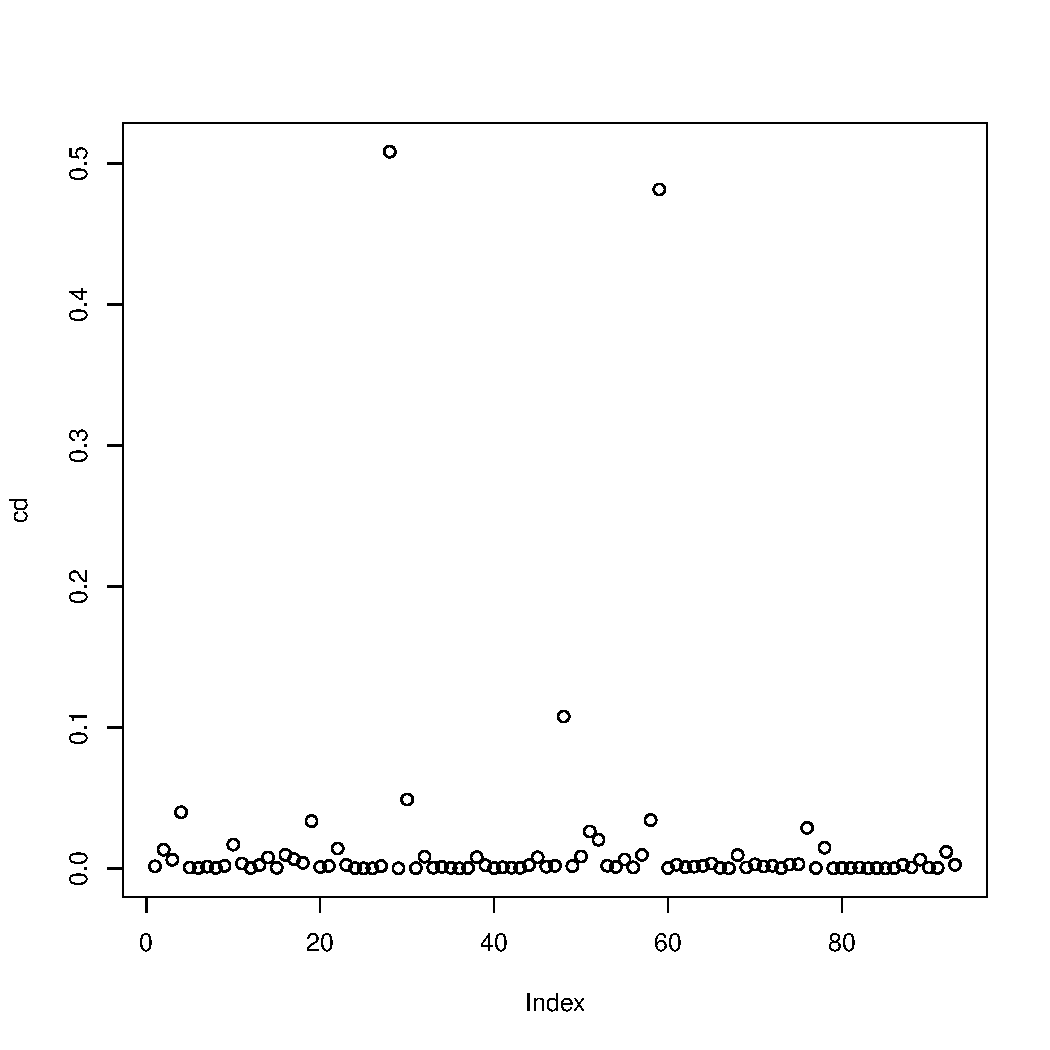
\includegraphics[width=\maxwidth]{figure/assumptions-unnamed-chunk-23-1} 

}


\end{knitrout}



\end{column}
\end{columns}

\end{frame}

\watermarkon %-----------------------------------------------------------------%

\begin{frame}{Outliers \& Leverages $\rightarrow$ Influential Points}

  Observations with high leverage or large (externally) studentized residuals
  are not necessarily influential.
  \vc
  \begin{itemize}
  \item High-leverage observations tend to be more influential than outliers.
    \vc
  \item The worst problems arise from observations that are both outliers and
    have high leverage.
  \end{itemize}
  \vb
  \emph{Measures of influence} simultaneously consider extremity in both $X$
  and $Y$ dimensions.
  \vc
  \begin{itemize}
  \item Observations with high measures of influence are very likely to cause
    problems.
  \end{itemize}

\end{frame}

%------------------------------------------------------------------------------%

\begin{frame}{Measures of Influence}

  Measures of influence come in two flavors.
  \vb
  \begin{enumerate}
  \item Global measures of influence
    \vc
    \begin{itemize}
    \item Cook's Distance
    \end{itemize}
    \vb
  \item Coefficient-specific measures of influence
    \vc
    \begin{itemize}
    \item DFBETAS
    \end{itemize}
  \end{enumerate}
  \vb
  All measures of influence use the same logic as the deleted residual.
  \vc
  \begin{itemize}
  \item Compare models estimated from the whole sample to models estimated from
    samples excluding individual observations.
  \end{itemize}
\end{frame}

%------------------------------------------------------------------------------%

\begin{frame}{Global Measures of Influence}

  Each observation gets a Cook's Distance value.
  \begin{align*}
    \textrm{Cook's} ~ D_n &= \frac{\sum_{n = 1}^N \left( \hat{Y}_n - \hat{Y}_{(n)} \right)^2}{\left(P + 1\right) \hat{\sigma}^2}\\[6pt]
                          &= (P + 1)^{-1} t_n^2 \frac{h_n}{1 - h_n}
  \end{align*}

  Each regression coefficient (including the intercept) gets a DFBETAS value for
  each observation.
  \begin{align*}
    \textrm{DFBETAS}_{np} = \frac{\hat{\beta}_p - \hat{\beta}_{p(n)}}{\textrm{SE}_{\hat{\beta}_{p(n)}}}
  \end{align*}

\end{frame}

\watermarkoff %----------------------------------------------------------------%

\begin{frame}[fragile]{Plots of Cook's Distance}

  \begin{columns}
    \begin{column}{0.5\textwidth}

      Index plots of Cook's distances can help spotlight the influential points.
      \vb
      \begin{itemize}
      \item Look for observations that clearly ``stand out from the crowd.''
      \end{itemize}

    \end{column}
    \begin{column}{0.5\textwidth}



\begin{knitrout}\footnotesize
\definecolor{shadecolor}{rgb}{0.878, 0.918, 0.933}\color{fgcolor}\begin{kframe}
\begin{alltt}
\hlstd{cd} \hlkwb{<-} \hlkwd{cooks.distance}\hlstd{(out1)}
\hlkwd{plot}\hlstd{(cd)}
\end{alltt}
\end{kframe}

{\centering 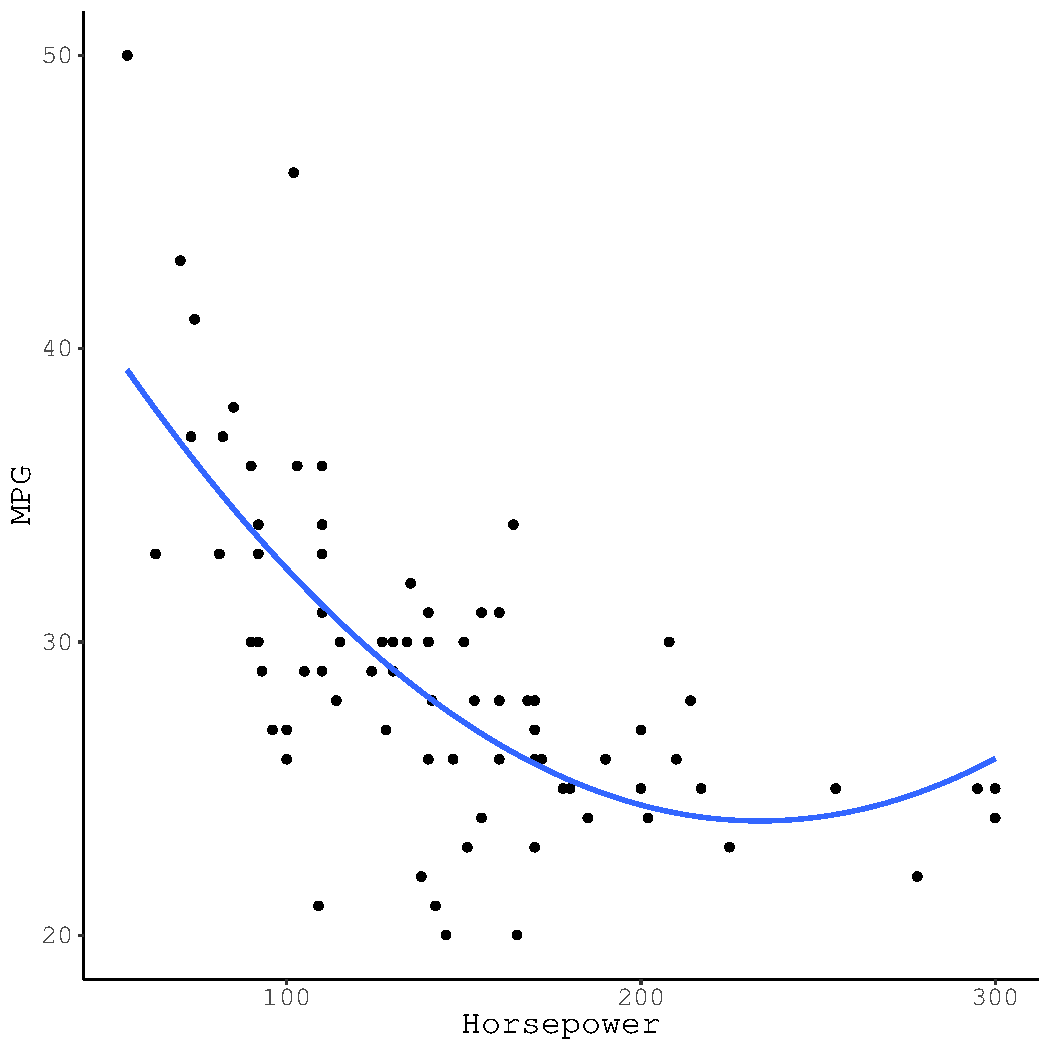
\includegraphics[width=\maxwidth]{figure/assumptions-unnamed-chunk-26-1} 

}


\end{knitrout}

\end{column}
\end{columns}

\end{frame}

%------------------------------------------------------------------------------%

\begin{frame}[fragile]{Plots of DFBETAS}

\begin{knitrout}\footnotesize
\definecolor{shadecolor}{rgb}{0.878, 0.918, 0.933}\color{fgcolor}\begin{kframe}
\begin{alltt}
\hlstd{dfb} \hlkwb{<-} \hlkwd{dfbetas}\hlstd{(out1)}
\hlkwd{plot}\hlstd{(dfb[ ,} \hlnum{1}\hlstd{],} \hlkwc{main} \hlstd{=} \hlstr{"Intercept"}\hlstd{)}
\hlkwd{plot}\hlstd{(dfb[ ,} \hlnum{2}\hlstd{],} \hlkwc{main} \hlstd{=} \hlstr{"Slope"}\hlstd{)}
\end{alltt}
\end{kframe}
\end{knitrout}

  \begin{columns}
    \begin{column}{0.5\textwidth}

\begin{knitrout}\footnotesize
\definecolor{shadecolor}{rgb}{0.878, 0.918, 0.933}\color{fgcolor}

{\centering 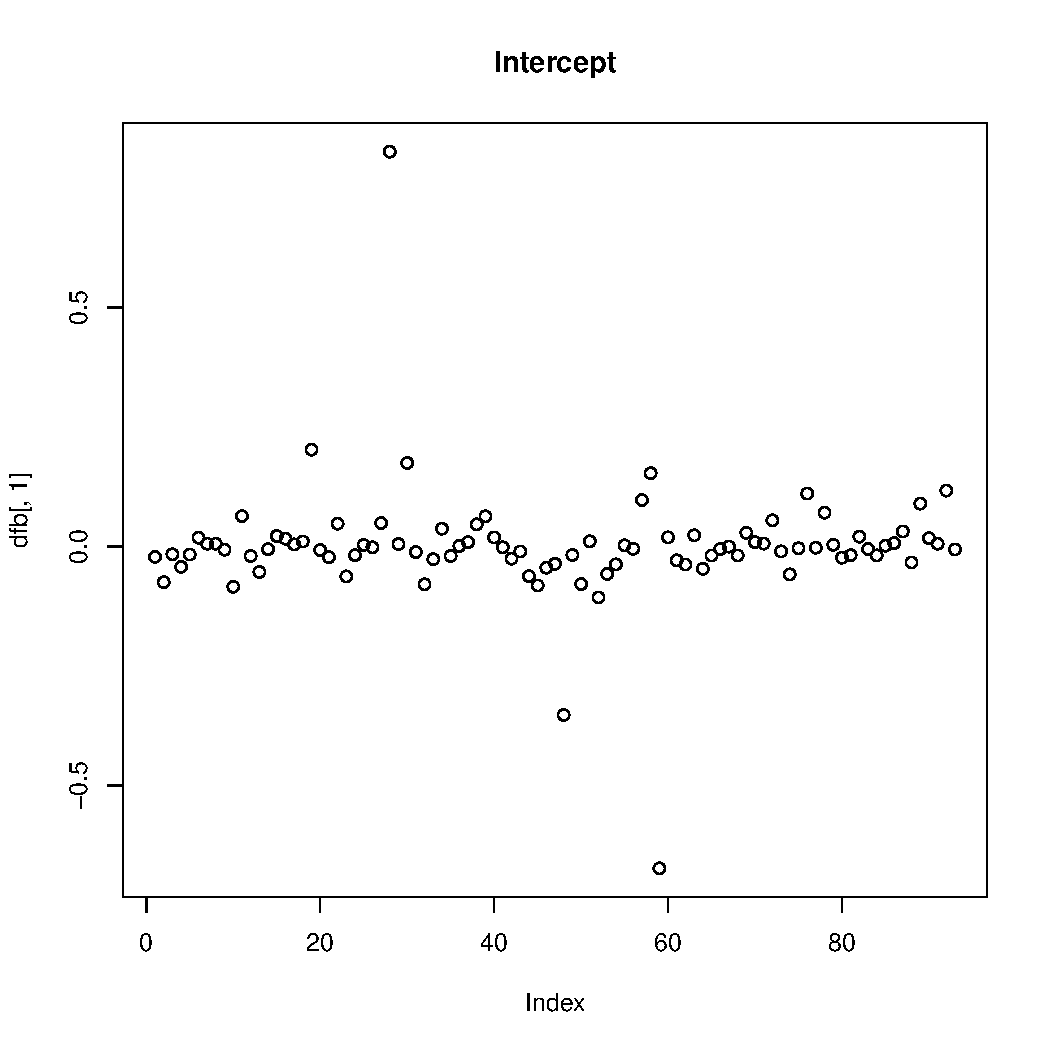
\includegraphics[width=\maxwidth]{figure/assumptions-unnamed-chunk-28-1} 

}


\end{knitrout}



\end{column}
\begin{column}{0.5\textwidth}

\begin{knitrout}\footnotesize
\definecolor{shadecolor}{rgb}{0.878, 0.918, 0.933}\color{fgcolor}

{\centering 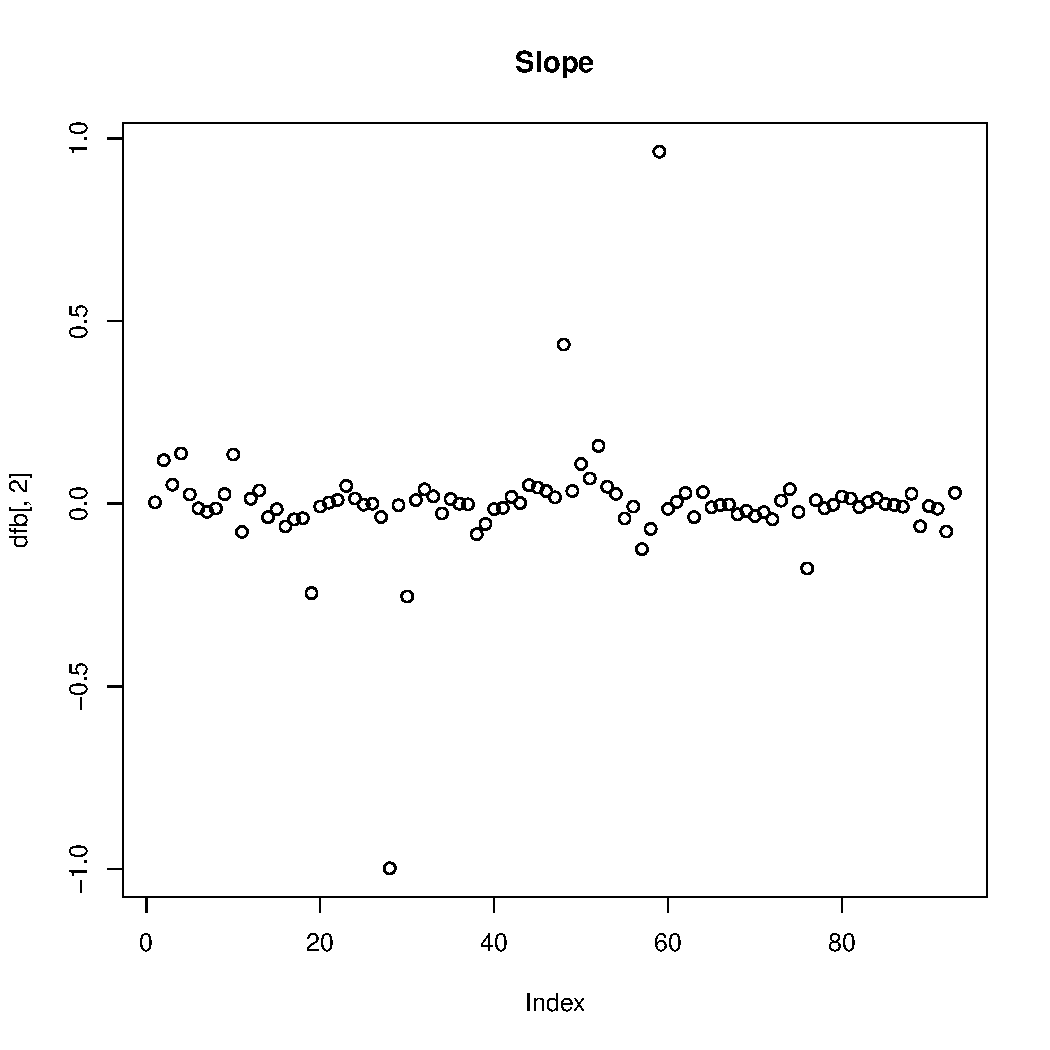
\includegraphics[width=\maxwidth]{figure/assumptions-unnamed-chunk-30-1} 

}


\end{knitrout}



\end{column}
\end{columns}

\end{frame}

%------------------------------------------------------------------------------%

\subsection{Treating Influential Observations}

%------------------------------------------------------------------------------%

\begin{frame}[fragile]{Removing Influential Observations}

\begin{knitrout}\footnotesize
\definecolor{shadecolor}{rgb}{0.878, 0.918, 0.933}\color{fgcolor}\begin{kframe}
\begin{alltt}
\hlstd{(maxD} \hlkwb{<-} \hlkwd{which.max}\hlstd{(cd))}
\end{alltt}
\begin{verbatim}
28 
28 
\end{verbatim}
\end{kframe}
\end{knitrout}

  \begin{columns}
    \begin{column}{0.5\textwidth}

      Observation number 28 was the most influential
      according to Cook's Distance.
      \vb
      \begin{itemize}
      \item Removing that observation has a small impact on the fitted
        regression line.
        \vc
      \item Influential observations don't only affect the regression line,
        though.
      \end{itemize}

    \end{column}

    \begin{column}{0.5\textwidth}

\begin{knitrout}\footnotesize
\definecolor{shadecolor}{rgb}{0.878, 0.918, 0.933}\color{fgcolor}

{\centering 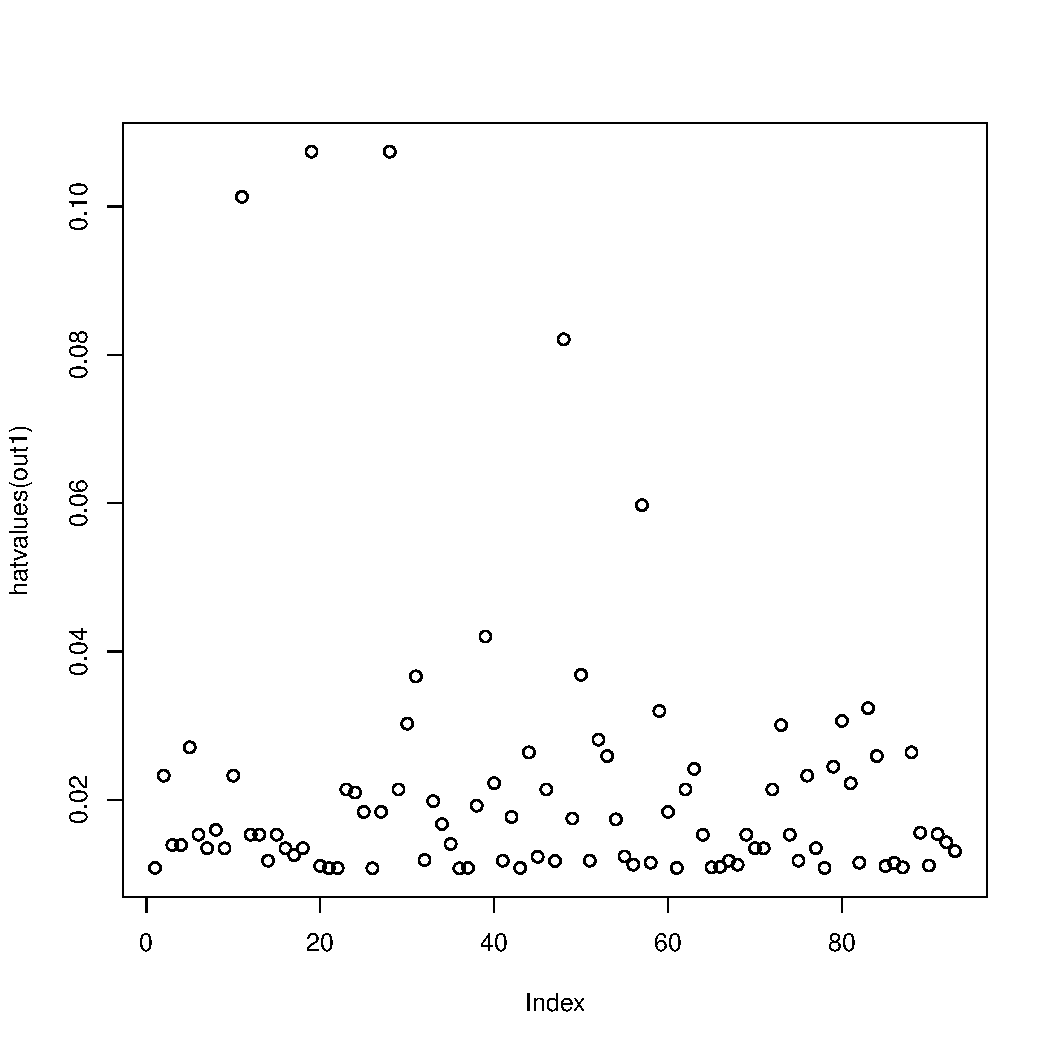
\includegraphics[width=\maxwidth]{figure/assumptions-unnamed-chunk-33-1} 

}


\end{knitrout}

\end{column}
\end{columns}

\end{frame}

%------------------------------------------------------------------------------%

\begin{frame}[fragile, allowframebreaks]{Removing Influential Observations}

\begin{knitrout}\footnotesize
\definecolor{shadecolor}{rgb}{0.878, 0.918, 0.933}\color{fgcolor}\begin{kframe}
\begin{alltt}
\hlcom{## Exclude the influential case:}
\hlstd{Cars93.2} \hlkwb{<-} \hlstd{Cars93[}\hlopt{-}\hlstd{maxD, ]}

\hlcom{## Fit model with reduced sample:}
\hlstd{out2} \hlkwb{<-} \hlkwd{lm}\hlstd{(Price} \hlopt{~} \hlstd{Horsepower,} \hlkwc{data} \hlstd{= Cars93.2)}

\hlkwd{round}\hlstd{(}\hlkwd{summary}\hlstd{(out1)}\hlopt{$}\hlstd{coefficients,} \hlnum{6}\hlstd{)}
\end{alltt}
\begin{verbatim}
             Estimate Std. Error   t value Pr(>|t|)
(Intercept) -1.398769   1.820016 -0.768548 0.444152
Horsepower   0.145371   0.011898 12.218325 0.000000
\end{verbatim}
\begin{alltt}
\hlkwd{round}\hlstd{(}\hlkwd{summary}\hlstd{(out2)}\hlopt{$}\hlstd{coefficients,} \hlnum{6}\hlstd{)}
\end{alltt}
\begin{verbatim}
             Estimate Std. Error   t value Pr(>|t|)
(Intercept) -2.837646   1.806418 -1.570868 0.119722
Horsepower   0.156750   0.011996 13.066942 0.000000
\end{verbatim}
\end{kframe}
\end{knitrout}

\pagebreak

\begin{knitrout}\footnotesize
\definecolor{shadecolor}{rgb}{0.878, 0.918, 0.933}\color{fgcolor}\begin{kframe}
\begin{alltt}
\hlkwd{partSummary}\hlstd{(out1,} \hlnum{2}\hlstd{)}
\end{alltt}
\begin{verbatim}
Residuals:
    Min      1Q  Median      3Q     Max 
-16.413  -2.792  -0.821   1.803  31.753 
\end{verbatim}
\begin{alltt}
\hlkwd{partSummary}\hlstd{(out2,} \hlnum{2}\hlstd{)}
\end{alltt}
\begin{verbatim}
Residuals:
     Min       1Q   Median       3Q      Max 
-11.4069  -3.0349  -0.5912   1.8530  30.7229 
\end{verbatim}
\end{kframe}
\end{knitrout}

\pagebreak

\begin{knitrout}\footnotesize
\definecolor{shadecolor}{rgb}{0.878, 0.918, 0.933}\color{fgcolor}\begin{kframe}
\begin{alltt}
\hlkwd{summary}\hlstd{(out1)[}\hlkwd{c}\hlstd{(}\hlstr{"sigma"}\hlstd{,} \hlstr{"r.squared"}\hlstd{,} \hlstr{"fstatistic"}\hlstd{)]} \hlopt
    \hlkwd{unlist}\hlstd{()} \hlopt
    \hlkwd{head}\hlstd{(}\hlnum{3}\hlstd{)}
\end{alltt}
\begin{verbatim}
           sigma        r.squared fstatistic.value 
        5.976953         0.621287       149.287468 
\end{verbatim}
\begin{alltt}
\hlkwd{summary}\hlstd{(out2)[}\hlkwd{c}\hlstd{(}\hlstr{"sigma"}\hlstd{,} \hlstr{"r.squared"}\hlstd{,} \hlstr{"fstatistic"}\hlstd{)]} \hlopt
    \hlkwd{unlist}\hlstd{()} \hlopt
    \hlkwd{head}\hlstd{(}\hlnum{3}\hlstd{)}
\end{alltt}
\begin{verbatim}
           sigma        r.squared fstatistic.value 
       5.7243112        0.6548351      170.7449721 
\end{verbatim}
\end{kframe}
\end{knitrout}

\end{frame}

%------------------------------------------------------------------------------%

\begin{frame}[fragile]{Removing Influential Observations}

\begin{knitrout}\footnotesize
\definecolor{shadecolor}{rgb}{0.878, 0.918, 0.933}\color{fgcolor}\begin{kframe}
\begin{alltt}
\hlstd{(maxDs} \hlkwb{<-} \hlkwd{sort}\hlstd{(cd)} \hlopt \hlkwd{names}\hlstd{()} \hlopt \hlkwd{tail}\hlstd{(}\hlnum{2}\hlstd{)} \hlopt \hlkwd{as.numeric}\hlstd{())}
\end{alltt}
\begin{verbatim}
[1] 59 28
\end{verbatim}
\end{kframe}
\end{knitrout}

  \begin{columns}
    \begin{column}{0.5\textwidth}

      If we remove the two most influential observations, 59 and
      28, the fitted regression line barely changes at all.
      \vc
      \begin{itemize}
      \item The influences of these two observations were counteracting one
        another.
      \item We're probably still better off, though.
      \end{itemize}

    \end{column}

    \begin{column}{0.5\textwidth}

\begin{knitrout}\footnotesize
\definecolor{shadecolor}{rgb}{0.878, 0.918, 0.933}\color{fgcolor}

{\centering 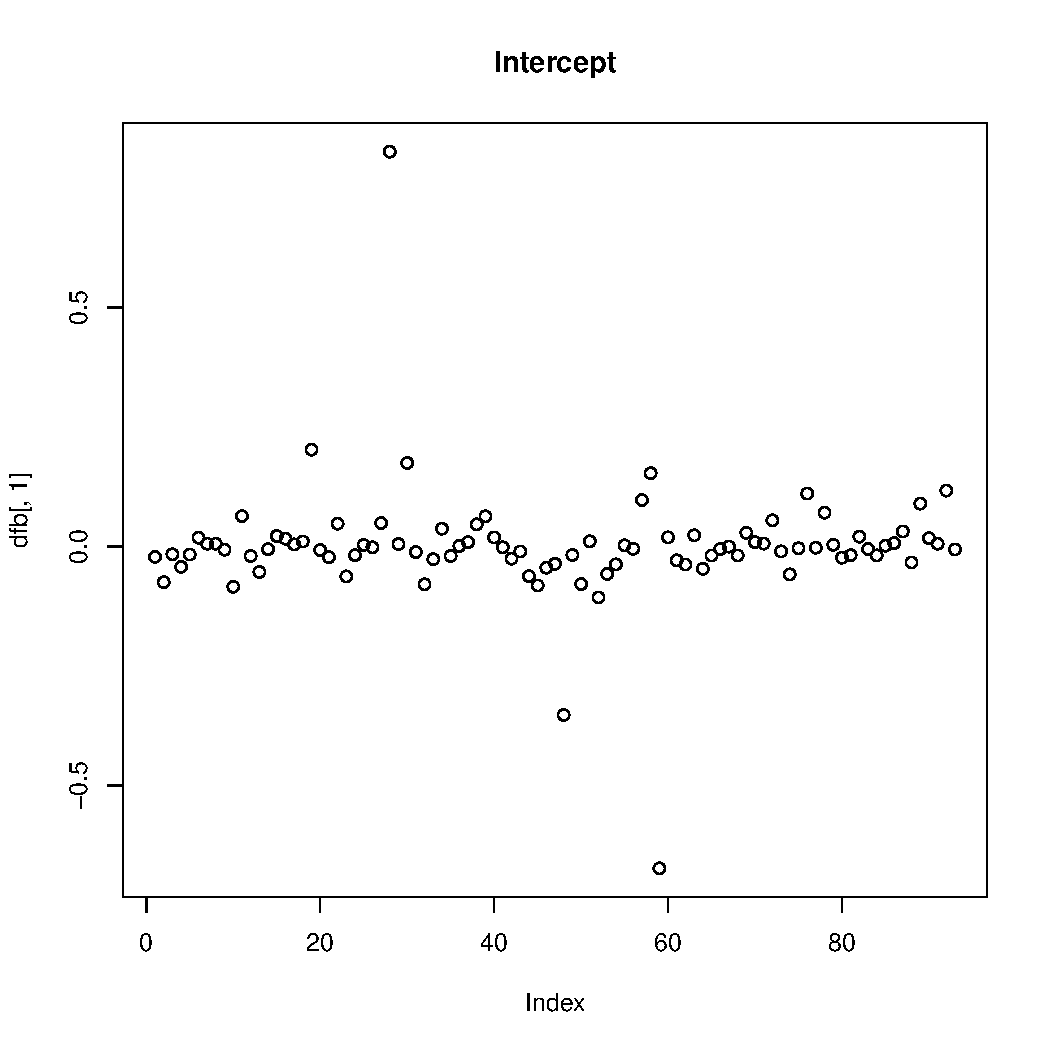
\includegraphics[width=\maxwidth]{figure/assumptions-unnamed-chunk-38-1} 

}


\end{knitrout}

\end{column}
\end{columns}

\end{frame}

%------------------------------------------------------------------------------%

\begin{frame}[fragile, allowframebreaks]{Removing Influential Observations}

\begin{knitrout}\footnotesize
\definecolor{shadecolor}{rgb}{0.878, 0.918, 0.933}\color{fgcolor}\begin{kframe}
\begin{alltt}
\hlcom{## Exclude influential cases:}
\hlstd{Cars93.2} \hlkwb{<-} \hlstd{Cars93[}\hlopt{-}\hlstd{maxDs, ]}

\hlcom{## Fit model with reduced sample:}
\hlstd{out2.2} \hlkwb{<-} \hlkwd{lm}\hlstd{(Price} \hlopt{~} \hlstd{Horsepower,} \hlkwc{data} \hlstd{= Cars93.2)}

\hlkwd{round}\hlstd{(}\hlkwd{summary}\hlstd{(out1)}\hlopt{$}\hlstd{coefficients,} \hlnum{6}\hlstd{)}
\end{alltt}
\begin{verbatim}
             Estimate Std. Error   t value Pr(>|t|)
(Intercept) -1.398769   1.820016 -0.768548 0.444152
Horsepower   0.145371   0.011898 12.218325 0.000000
\end{verbatim}
\begin{alltt}
\hlkwd{round}\hlstd{(}\hlkwd{summary}\hlstd{(out2.2)}\hlopt{$}\hlstd{coefficients,} \hlnum{6}\hlstd{)}
\end{alltt}
\begin{verbatim}
             Estimate Std. Error   t value Pr(>|t|)
(Intercept) -1.695315   1.494767 -1.134166  0.25977
Horsepower   0.146277   0.009986 14.648807  0.00000
\end{verbatim}
\end{kframe}
\end{knitrout}

\pagebreak

\begin{knitrout}\footnotesize
\definecolor{shadecolor}{rgb}{0.878, 0.918, 0.933}\color{fgcolor}\begin{kframe}
\begin{alltt}
\hlkwd{partSummary}\hlstd{(out1,} \hlnum{2}\hlstd{)}
\end{alltt}
\begin{verbatim}
Residuals:
    Min      1Q  Median      3Q     Max 
-16.413  -2.792  -0.821   1.803  31.753 
\end{verbatim}
\begin{alltt}
\hlkwd{partSummary}\hlstd{(out2.2,} \hlnum{2}\hlstd{)}
\end{alltt}
\begin{verbatim}
Residuals:
     Min       1Q   Median       3Q      Max 
-10.3079  -2.5786  -0.6084   1.9775  14.5793 
\end{verbatim}
\end{kframe}
\end{knitrout}

\pagebreak

\begin{knitrout}\footnotesize
\definecolor{shadecolor}{rgb}{0.878, 0.918, 0.933}\color{fgcolor}\begin{kframe}
\begin{alltt}
\hlkwd{summary}\hlstd{(out1)[}\hlkwd{c}\hlstd{(}\hlstr{"sigma"}\hlstd{,} \hlstr{"r.squared"}\hlstd{,} \hlstr{"fstatistic"}\hlstd{)]} \hlopt
    \hlkwd{unlist}\hlstd{()} \hlopt
    \hlkwd{head}\hlstd{(}\hlnum{3}\hlstd{)}
\end{alltt}
\begin{verbatim}
           sigma        r.squared fstatistic.value 
        5.976953         0.621287       149.287468 
\end{verbatim}
\begin{alltt}
\hlkwd{summary}\hlstd{(out2.2)[}\hlkwd{c}\hlstd{(}\hlstr{"sigma"}\hlstd{,} \hlstr{"r.squared"}\hlstd{,} \hlstr{"fstatistic"}\hlstd{)]} \hlopt
    \hlkwd{unlist}\hlstd{()} \hlopt
    \hlkwd{head}\hlstd{(}\hlnum{3}\hlstd{)}
\end{alltt}
\begin{verbatim}
           sigma        r.squared fstatistic.value 
       4.7053314        0.7068391      214.5875491 
\end{verbatim}
\end{kframe}
\end{knitrout}

\end{frame}

\watermarkon %-----------------------------------------------------------------%

\begin{frame}{Treating Influential Points}

  The most common way to address influential observations is simply to delete
  them and refit the model.
  \vc
  \begin{itemize}
  \item This approach is often effective---and always simple---but it is not
    fool-proof.
  \vc
  \item Although an observation is influential, we may not be able to justify
    excluding it from the analysis.
  \end{itemize}
  \vb
  Robust regression procedures can estimate the model directly in the
  presence of influential observations.
  \vc
  \begin{itemize}
  \item Observations in the tails of the distribution are weighted less in the
    estimation process, so outliers and high-leverage points cannot exert
    substantial influence on the fit.
  \end{itemize}

\end{frame}

%------------------------------------------------------------------------------%

\end{document}
